\documentclass{slides}
\usepackage{xspace}
\usepackage{nth}
\usepackage{fontawesome}
\usepackage{hyperref}
\hypersetup{
    colorlinks = true,
    urlcolor = blue
}

\title[Bayesian Inference]{Bayesian inference in Normal distributions}
\author[Andrews]{Mark Andrews \\ $\phantom{foo}$ \\ Psychology, Nottingham Trent University \\ $\phantom{foo}$ \\ \faEnvelopeO \  \texttt{mark.andrews@ntu.ac.uk} \\ $\phantom{foo}$ \\ \faTwitter \href{https://twitter.com/xmjandrews}{@xmjandrews}, \faTwitter \href{https://twitter.com/priorexposure}{@priorexposure}\\ $\phantom{foo}$ \\ \faGithub \ \url{https://github.com/lawsofthought/psbayes}}

\date{December, 2018}

\begin{document}
{
	\begin{frame}
		\titlepage
	\end{frame}
}


\begin{frame}
	\frametitle{Inference in normal distributions}
	\begin{itemize}
		\item The univariate normal, or Gaussian, probability distribution with mean $\mu$ and variance $\sigma^2$ has the density
			\[
				\Prob{x\given\mu,\sigma} = \frac{1}{\sqrt{2\pi\sigma^2}}e^{-\frac{(x-\mu)^2}{2\sigma^2}}.
			\]
		\item A random variable $x$ that is normally distributed with mean $\mu$ and variance $\sigma^2$ can be written
			\[
				x \sim \textrm{N}(\mu, \sigma^2).
			\]

	\end{itemize}
\end{frame}

\begin{frame}
	\frametitle{Inference in normal distributions}
	\begin{itemize}
		\item A common elementary data analysis problem is when we
			observe $n$ iid samples from $\textrm{N}(\mu, \sigma^2)$, where
			$\mu$ and $\sigma^2$ are unknown, and we aim to infer
			$\mu$.

		\item In other words, we observe
			\[D = x_1, x_2 \cdots x_n,\]
			where we assume
			\[x_i \sim \textrm{N}(\mu, \sigma^2),\quad\text{for $i \in 1,2\cdots n$},\]
		      where both $\mu$ and $\sigma^2$ are unknown, and we aim to infer the value of $\mu$. 
		\item In other words, we aim to determine the posterior distribution
		      \[
			\Prob{\mu \given D}.
		      \]
	\end{itemize}
\end{frame}


\begin{frame}
	\frametitle{Likelihood of $\mu$ and $\sigma^2$}
	\begin{itemize}
		\item The likelihood of $\mu$ and $\sigma^2$ given $D$ is 
			\begin{align*}
				\Prob{x_1, x_2 \cdots x_n \given \mu, \sigma^2} &= \prod_{i=1}^n \Prob{x_i \given \mu, \sigma^2},\\
				&= \prod_{i=1}^n \frac{1}{\sqrt{2\pi\sigma^2}}e^{-\frac{(x_i-\mu)^2}{2\sigma^2}},\\
				&= \left(\frac{1}{\sqrt{2\pi\sigma^2}}\right)^n e^{\left(-\tfrac{1}{2\sigma^2}\sum_{i=1}^{n}(x_i - \mu)^2\right)},\\
				&\propto \sigma^{-n} e^{\left( -\tfrac{1}{2\sigma^2}\left[n s^2 + n(\bar{x}-\mu)^2\right] \right)},
			\end{align*}
			with \[
				\bar{x} \doteq \tfrac{1}{n} \sum_{i=1}^n x_i, \quad s^2 \doteq \tfrac{1}{n} \sum_{i=1}^n (x_i - \bar{x})^2.
			\]
	\end{itemize}

\end{frame}

\begin{frame}
	\frametitle{Likelihood of $\mu$ and $\sigma^2$}

	\hspace*{-5mm}
	% Created by tikzDevice version 0.12 on 2018-12-03 08:01:46
% !TEX encoding = UTF-8 Unicode
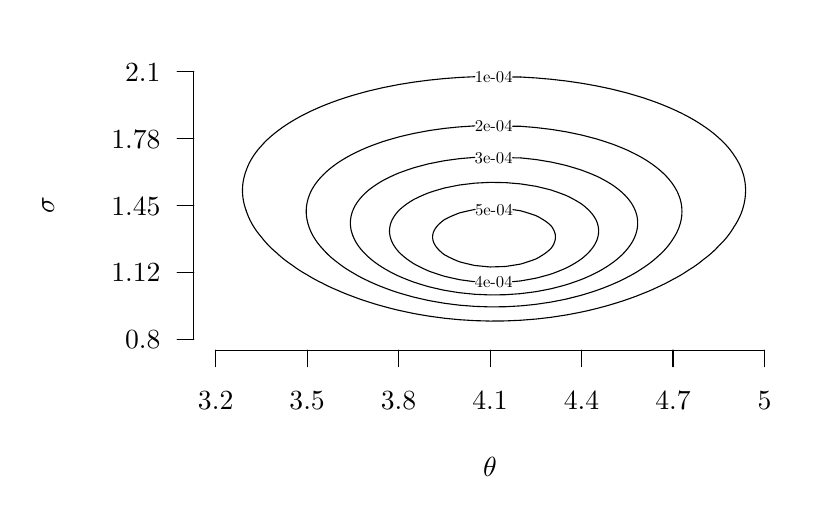
\begin{tikzpicture}[x=1pt,y=1pt]
\definecolor{fillColor}{RGB}{255,255,255}
\path[use as bounding box,fill=fillColor,fill opacity=0.00] (0,0) rectangle (274.17,164.50);
\begin{scope}
\path[clip] ( 60.00, 48.00) rectangle (274.17,152.50);
\definecolor{drawColor}{RGB}{0,0,0}

\path[draw=drawColor,line width= 0.4pt,line join=round,line cap=round] ( 78.95, 98.43) --
	( 78.83, 98.76) --
	( 78.58, 99.51) --
	( 78.36,100.25) --
	( 78.17,101.00) --
	( 78.01,101.74) --
	( 77.88,102.48) --
	( 77.77,103.23) --
	( 77.70,103.97) --
	( 77.65,104.72) --
	( 77.62,105.46) --
	( 77.63,106.21) --
	( 77.66,106.95) --
	( 77.72,107.69) --
	( 77.81,108.44) --
	( 77.93,109.18) --
	( 78.08,109.93) --
	( 78.25,110.67) --
	( 78.46,111.42) --
	( 78.69,112.16) --
	( 78.95,112.87) --
	( 78.96,112.90) --
	( 79.23,113.65) --
	( 79.54,114.39) --
	( 79.87,115.14) --
	( 80.24,115.88) --
	( 80.64,116.63) --
	( 81.08,117.37) --
	( 81.55,118.11) --
	( 82.06,118.86) --
	( 82.60,119.60) --
	( 83.19,120.35) --
	( 83.82,121.09) --
	( 84.46,121.81) --
	( 84.48,121.84) --
	( 85.15,122.58) --
	( 85.87,123.33) --
	( 86.63,124.07) --
	( 87.44,124.81) --
	( 88.30,125.56) --
	( 89.20,126.30) --
	( 89.97,126.90) --
	( 90.16,127.05) --
	( 91.14,127.79) --
	( 92.17,128.54) --
	( 93.27,129.28) --
	( 94.42,130.02) --
	( 95.47,130.67) --
	( 95.64,130.77) --
	( 96.90,131.51) --
	( 98.23,132.26) --
	( 99.64,133.00) --
	(100.98,133.68) --
	(101.11,133.75) --
	(102.67,134.49) --
	(104.30,135.23) --
	(106.03,135.98) --
	(106.49,136.17) --
	(107.86,136.72) --
	(109.79,137.47) --
	(111.83,138.21) --
	(112.00,138.27) --
	(114.04,138.96) --
	(116.36,139.70) --
	(117.51,140.05) --
	(118.88,140.44) --
	(121.58,141.19) --
	(123.02,141.57) --
	(124.53,141.93) --
	(127.74,142.68) --
	(128.53,142.86) --
	(131.37,143.42) --
	(134.03,143.94) --
	(135.43,144.17) --
	(139.54,144.83) --
	(140.16,144.91) --
	(145.05,145.55) --
	(146.06,145.65) --
	(150.56,146.11) --
	(154.46,146.40) --
	(156.07,146.52) --
	(161.58,146.78);

\path[draw=drawColor,line width= 0.4pt,line join=round,line cap=round] (178.10,146.67) --
	(182.63,146.40) --
	(183.61,146.34) --
	(189.12,145.86) --
	(190.93,145.65) --
	(194.63,145.23) --
	(196.82,144.91) --
	(200.14,144.42) --
	(201.60,144.17) --
	(205.64,143.44) --
	(205.73,143.42) --
	(209.26,142.68) --
	(211.15,142.27) --
	(212.51,141.93) --
	(215.45,141.19) --
	(216.66,140.87) --
	(218.16,140.44) --
	(220.66,139.70) --
	(222.17,139.24) --
	(223.01,138.96) --
	(225.18,138.21) --
	(227.25,137.47) --
	(227.68,137.31) --
	(229.18,136.72) --
	(231.00,135.98) --
	(232.73,135.23) --
	(233.19,135.03) --
	(234.37,134.49) --
	(235.92,133.75) --
	(237.40,133.00) --
	(238.70,132.31) --
	(238.80,132.26) --
	(240.14,131.51) --
	(241.41,130.77) --
	(242.61,130.02) --
	(243.75,129.28) --
	(244.20,128.97) --
	(244.85,128.54) --
	(245.90,127.79) --
	(246.90,127.05) --
	(247.84,126.30) --
	(248.73,125.56) --
	(249.57,124.81) --
	(249.71,124.68) --
	(250.39,124.07) --
	(251.17,123.33) --
	(251.90,122.58) --
	(252.59,121.84) --
	(253.24,121.09) --
	(253.85,120.35) --
	(254.41,119.60) --
	(254.94,118.86) --
	(255.22,118.43) --
	(255.44,118.11) --
	(255.93,117.37) --
	(256.38,116.63) --
	(256.80,115.88) --
	(257.19,115.14) --
	(257.54,114.39) --
	(257.85,113.65) --
	(258.14,112.90) --
	(258.39,112.16) --
	(258.62,111.42) --
	(258.82,110.67) --
	(258.98,109.93) --
	(259.12,109.18) --
	(259.23,108.44) --
	(259.32,107.69) --
	(259.37,106.95) --
	(259.41,106.21) --
	(259.41,105.46) --
	(259.39,104.72) --
	(259.34,103.97) --
	(259.27,103.23) --
	(259.17,102.48) --
	(259.05,101.74) --
	(258.90,101.00) --
	(258.72,100.25) --
	(258.52, 99.51) --
	(258.29, 98.76) --
	(258.04, 98.02) --
	(257.76, 97.27) --
	(257.44, 96.53) --
	(257.10, 95.79) --
	(256.73, 95.04) --
	(256.32, 94.30) --
	(255.89, 93.55) --
	(255.41, 92.81) --
	(255.22, 92.53) --
	(254.95, 92.06) --
	(254.48, 91.32) --
	(253.99, 90.58) --
	(253.45, 89.83) --
	(252.89, 89.09) --
	(252.28, 88.34) --
	(251.63, 87.60) --
	(250.94, 86.85) --
	(250.21, 86.11) --
	(249.71, 85.64) --
	(249.46, 85.36) --
	(248.75, 84.62) --
	(248.00, 83.88) --
	(247.19, 83.13) --
	(246.33, 82.39) --
	(245.41, 81.64) --
	(244.43, 80.90) --
	(244.20, 80.74) --
	(243.50, 80.15) --
	(242.55, 79.41) --
	(241.54, 78.67) --
	(240.45, 77.92) --
	(239.28, 77.18) --
	(238.70, 76.83) --
	(238.12, 76.43) --
	(236.98, 75.69) --
	(235.74, 74.94) --
	(234.41, 74.20) --
	(233.19, 73.56) --
	(233.00, 73.46) --
	(231.67, 72.71) --
	(230.23, 71.97) --
	(228.66, 71.22) --
	(227.68, 70.78) --
	(227.06, 70.48) --
	(225.45, 69.73) --
	(223.70, 68.99) --
	(222.17, 68.39) --
	(221.82, 68.25) --
	(219.97, 67.50) --
	(217.93, 66.76) --
	(216.66, 66.33) --
	(215.78, 66.01) --
	(213.54, 65.27) --
	(211.15, 64.55) --
	(211.07, 64.52) --
	(208.51, 63.78) --
	(205.67, 63.04) --
	(205.64, 63.03) --
	(202.60, 62.29) --
	(200.14, 61.75) --
	(199.15, 61.55) --
	(195.25, 60.80) --
	(194.63, 60.69) --
	(190.56, 60.06) --
	(189.12, 59.84) --
	(184.54, 59.31) --
	(183.61, 59.21) --
	(178.10, 58.77) --
	(173.48, 58.57) --
	(172.59, 58.53) --
	(167.09, 58.48) --
	(163.90, 58.57) --
	(161.58, 58.63) --
	(156.07, 58.97) --
	(152.57, 59.31) --
	(150.56, 59.51) --
	(146.49, 60.06) --
	(145.05, 60.26) --
	(141.82, 60.80) --
	(139.54, 61.21) --
	(137.88, 61.55) --
	(134.45, 62.29) --
	(134.03, 62.38) --
	(131.34, 63.04) --
	(128.56, 63.78) --
	(128.53, 63.79) --
	(125.92, 64.52) --
	(123.54, 65.27) --
	(123.02, 65.44) --
	(121.23, 66.01) --
	(119.10, 66.76) --
	(117.51, 67.36) --
	(117.12, 67.50) --
	(115.15, 68.25) --
	(113.35, 68.99) --
	(112.00, 69.59) --
	(111.65, 69.73) --
	(109.92, 70.48) --
	(108.34, 71.22) --
	(106.88, 71.97) --
	(106.49, 72.18) --
	(105.38, 72.71) --
	(103.94, 73.46) --
	(102.61, 74.20) --
	(101.38, 74.94) --
	(100.98, 75.19) --
	(100.10, 75.69) --
	( 98.85, 76.43) --
	( 97.69, 77.18) --
	( 96.61, 77.92) --
	( 95.60, 78.67) --
	( 95.47, 78.76) --
	( 94.51, 79.41) --
	( 93.48, 80.15) --
	( 92.51, 80.90) --
	( 91.61, 81.64) --
	( 90.76, 82.39) --
	( 89.97, 83.13) --
	( 89.96, 83.13) --
	( 89.08, 83.88) --
	( 88.25, 84.62) --
	( 87.48, 85.36) --
	( 86.76, 86.11) --
	( 86.08, 86.85) --
	( 85.44, 87.60) --
	( 84.84, 88.34) --
	( 84.46, 88.84) --
	( 84.24, 89.09) --
	( 83.62, 89.83) --
	( 83.04, 90.58) --
	( 82.50, 91.32) --
	( 82.00, 92.06) --
	( 81.53, 92.81) --
	( 81.09, 93.55) --
	( 80.69, 94.30) --
	( 80.31, 95.04) --
	( 79.96, 95.79) --
	( 79.64, 96.53) --
	( 79.35, 97.27) --
	( 79.08, 98.02) --
	( 78.95, 98.43);

\path[draw=drawColor,line width= 0.4pt,line join=round,line cap=round] (175.24,146.69) -- (178.10,146.67);

\node[text=drawColor,rotate= -0.36,anchor=base west,inner sep=0pt, outer sep=0pt, scale=  0.60] at (161.56,144.71) { 1e-04 };

\path[draw=drawColor,line width= 0.4pt,line join=round,line cap=round] (100.98, 94.98) --
	(100.97, 95.04) --
	(100.83, 95.79) --
	(100.74, 96.53) --
	(100.68, 97.27) --
	(100.65, 98.02) --
	(100.67, 98.76) --
	(100.72, 99.51) --
	(100.80,100.25) --
	(100.93,101.00) --
	(100.98,101.24) --
	(101.09,101.74) --
	(101.28,102.48) --
	(101.51,103.23) --
	(101.78,103.97) --
	(102.09,104.72) --
	(102.44,105.46) --
	(102.83,106.21) --
	(103.27,106.95) --
	(103.75,107.69) --
	(104.28,108.44) --
	(104.85,109.18) --
	(105.48,109.93) --
	(106.16,110.67) --
	(106.49,111.02) --
	(106.88,111.42) --
	(107.65,112.16) --
	(108.47,112.90) --
	(109.36,113.65) --
	(110.31,114.39) --
	(111.32,115.14) --
	(112.00,115.61) --
	(112.40,115.88) --
	(113.56,116.63) --
	(114.79,117.37) --
	(116.10,118.11) --
	(117.49,118.86) --
	(117.51,118.87) --
	(119.01,119.60) --
	(120.62,120.35) --
	(122.32,121.09) --
	(123.02,121.38) --
	(124.19,121.84) --
	(126.21,122.58) --
	(128.35,123.33) --
	(128.53,123.39) --
	(130.78,124.07) --
	(133.37,124.81) --
	(134.03,125.00) --
	(136.36,125.56) --
	(139.54,126.29) --
	(139.60,126.30) --
	(143.57,127.05) --
	(145.05,127.32) --
	(148.38,127.79) --
	(150.56,128.10) --
	(154.89,128.54) --
	(156.07,128.65) --
	(161.58,129.01);

\path[draw=drawColor,line width= 0.4pt,line join=round,line cap=round] (178.10,128.86) --
	(182.11,128.54) --
	(183.61,128.41) --
	(188.77,127.79) --
	(189.12,127.75) --
	(193.48,127.05) --
	(194.63,126.86) --
	(197.34,126.30) --
	(200.14,125.71) --
	(200.73,125.56) --
	(203.62,124.81) --
	(205.64,124.27) --
	(206.29,124.07) --
	(208.64,123.33) --
	(210.86,122.58) --
	(211.15,122.48) --
	(212.84,121.84) --
	(214.69,121.09) --
	(216.44,120.35) --
	(216.66,120.25) --
	(218.03,119.60) --
	(219.53,118.86) --
	(220.93,118.11) --
	(222.17,117.42) --
	(222.26,117.37) --
	(223.48,116.63) --
	(224.63,115.88) --
	(225.71,115.14) --
	(226.72,114.39) --
	(227.67,113.65) --
	(227.68,113.64) --
	(228.56,112.90) --
	(229.39,112.16) --
	(230.17,111.42) --
	(230.89,110.67) --
	(231.56,109.93) --
	(232.17,109.18) --
	(232.74,108.44) --
	(233.19,107.80) --
	(233.26,107.69) --
	(233.75,106.95) --
	(234.20,106.21) --
	(234.60,105.46) --
	(234.96,104.72) --
	(235.27,103.97) --
	(235.55,103.23) --
	(235.79,102.48) --
	(235.99,101.74) --
	(236.15,101.00) --
	(236.27,100.25) --
	(236.35, 99.51) --
	(236.40, 98.76) --
	(236.42, 98.02) --
	(236.40, 97.27) --
	(236.34, 96.53) --
	(236.25, 95.79) --
	(236.12, 95.04) --
	(235.96, 94.30) --
	(235.76, 93.55) --
	(235.52, 92.81) --
	(235.25, 92.06) --
	(234.94, 91.32) --
	(234.60, 90.58) --
	(234.21, 89.83) --
	(233.78, 89.09) --
	(233.31, 88.34) --
	(233.19, 88.16) --
	(232.83, 87.60) --
	(232.32, 86.85) --
	(231.78, 86.11) --
	(231.18, 85.36) --
	(230.55, 84.62) --
	(229.86, 83.88) --
	(229.12, 83.13) --
	(228.33, 82.39) --
	(227.68, 81.82) --
	(227.50, 81.64) --
	(226.66, 80.90) --
	(225.77, 80.15) --
	(224.82, 79.41) --
	(223.80, 78.67) --
	(222.71, 77.92) --
	(222.17, 77.58) --
	(221.59, 77.18) --
	(220.43, 76.43) --
	(219.19, 75.69) --
	(217.86, 74.94) --
	(216.66, 74.32) --
	(216.44, 74.20) --
	(214.99, 73.46) --
	(213.44, 72.71) --
	(211.76, 71.97) --
	(211.15, 71.71) --
	(210.00, 71.22) --
	(208.12, 70.48) --
	(206.08, 69.73) --
	(205.64, 69.58) --
	(203.89, 68.99) --
	(201.50, 68.25) --
	(200.14, 67.84) --
	(198.87, 67.50) --
	(195.93, 66.76) --
	(194.63, 66.44) --
	(192.54, 66.01) --
	(189.12, 65.35) --
	(188.61, 65.27) --
	(183.61, 64.53) --
	(183.59, 64.52) --
	(178.10, 63.97) --
	(174.75, 63.78) --
	(172.59, 63.66) --
	(167.09, 63.60) --
	(161.86, 63.78) --
	(161.58, 63.79) --
	(156.07, 64.22) --
	(153.64, 64.52) --
	(150.56, 64.92) --
	(148.49, 65.27) --
	(145.05, 65.88) --
	(144.44, 66.01) --
	(141.12, 66.76) --
	(139.54, 67.13) --
	(138.16, 67.50) --
	(135.54, 68.25) --
	(134.03, 68.70) --
	(133.14, 68.99) --
	(130.95, 69.73) --
	(128.93, 70.48) --
	(128.53, 70.64) --
	(127.03, 71.22) --
	(125.26, 71.97) --
	(123.62, 72.71) --
	(123.02, 73.00) --
	(122.05, 73.46) --
	(120.56, 74.20) --
	(119.17, 74.94) --
	(117.89, 75.69) --
	(117.51, 75.92) --
	(116.62, 76.43) --
	(115.41, 77.18) --
	(114.29, 77.92) --
	(113.24, 78.67) --
	(112.26, 79.41) --
	(112.00, 79.62) --
	(111.29, 80.15) --
	(110.35, 80.90) --
	(109.48, 81.64) --
	(108.67, 82.39) --
	(107.92, 83.13) --
	(107.21, 83.88) --
	(106.55, 84.62) --
	(106.49, 84.69) --
	(105.88, 85.36) --
	(105.26, 86.11) --
	(104.69, 86.85) --
	(104.15, 87.60) --
	(103.67, 88.34) --
	(103.22, 89.09) --
	(102.81, 89.83) --
	(102.44, 90.58) --
	(102.11, 91.32) --
	(101.81, 92.06) --
	(101.55, 92.81) --
	(101.32, 93.55) --
	(101.13, 94.30) --
	(100.98, 94.98);

\path[draw=drawColor,line width= 0.4pt,line join=round,line cap=round] (175.24,128.89) -- (178.10,128.86);

\node[text=drawColor,rotate= -0.50,anchor=base west,inner sep=0pt, outer sep=0pt, scale=  0.60] at (161.56,126.94) { 2e-04 };

\path[draw=drawColor,line width= 0.4pt,line join=round,line cap=round] (117.51, 89.33) --
	(117.32, 89.83) --
	(117.08, 90.58) --
	(116.89, 91.32) --
	(116.75, 92.06) --
	(116.66, 92.81) --
	(116.61, 93.55) --
	(116.61, 94.30) --
	(116.66, 95.04) --
	(116.76, 95.79) --
	(116.90, 96.53) --
	(117.09, 97.27) --
	(117.34, 98.02) --
	(117.51, 98.46) --
	(117.63, 98.76) --
	(117.97, 99.51) --
	(118.37,100.25) --
	(118.83,101.00) --
	(119.34,101.74) --
	(119.91,102.48) --
	(120.54,103.23) --
	(121.23,103.97) --
	(121.99,104.72) --
	(122.81,105.46) --
	(123.02,105.64) --
	(123.73,106.21) --
	(124.73,106.95) --
	(125.81,107.69) --
	(126.97,108.44) --
	(128.22,109.18) --
	(128.53,109.36) --
	(129.63,109.93) --
	(131.15,110.67) --
	(132.79,111.42) --
	(134.03,111.95) --
	(134.58,112.16) --
	(136.64,112.90) --
	(138.83,113.65) --
	(139.54,113.88) --
	(141.40,114.39) --
	(144.25,115.14) --
	(145.05,115.34) --
	(147.77,115.88) --
	(150.56,116.42) --
	(152.06,116.63) --
	(156.07,117.17) --
	(158.38,117.37) --
	(161.58,117.64);

\path[draw=drawColor,line width= 0.4pt,line join=round,line cap=round] (178.10,117.45) --
	(178.84,117.37) --
	(183.61,116.85) --
	(184.99,116.63) --
	(189.12,115.94) --
	(189.39,115.88) --
	(192.73,115.14) --
	(194.63,114.69) --
	(195.67,114.39) --
	(198.16,113.65) --
	(200.14,113.02) --
	(200.46,112.90) --
	(202.41,112.16) --
	(204.24,111.42) --
	(205.64,110.81) --
	(205.93,110.67) --
	(207.40,109.93) --
	(208.78,109.18) --
	(210.07,108.44) --
	(211.15,107.76) --
	(211.26,107.69) --
	(212.31,106.95) --
	(213.30,106.21) --
	(214.20,105.46) --
	(215.04,104.72) --
	(215.81,103.97) --
	(216.51,103.23) --
	(216.66,103.05) --
	(217.14,102.48) --
	(217.70,101.74) --
	(218.21,101.00) --
	(218.67,100.25) --
	(219.06, 99.51) --
	(219.41, 98.76) --
	(219.70, 98.02) --
	(219.94, 97.27) --
	(220.14, 96.53) --
	(220.28, 95.79) --
	(220.37, 95.04) --
	(220.42, 94.30) --
	(220.42, 93.55) --
	(220.38, 92.81) --
	(220.29, 92.06) --
	(220.15, 91.32) --
	(219.96, 90.58) --
	(219.73, 89.83) --
	(219.46, 89.09) --
	(219.13, 88.34) --
	(218.76, 87.60) --
	(218.33, 86.85) --
	(217.86, 86.11) --
	(217.33, 85.36) --
	(216.75, 84.62) --
	(216.66, 84.52) --
	(216.13, 83.88) --
	(215.45, 83.13) --
	(214.72, 82.39) --
	(213.92, 81.64) --
	(213.06, 80.90) --
	(212.13, 80.15) --
	(211.15, 79.43) --
	(211.13, 79.41) --
	(210.07, 78.67) --
	(208.92, 77.92) --
	(207.70, 77.18) --
	(206.38, 76.43) --
	(205.64, 76.05) --
	(204.95, 75.69) --
	(203.40, 74.94) --
	(201.74, 74.20) --
	(200.14, 73.53) --
	(199.94, 73.46) --
	(197.91, 72.71) --
	(195.72, 71.97) --
	(194.63, 71.62) --
	(193.22, 71.22) --
	(190.39, 70.48) --
	(189.12, 70.16) --
	(186.98, 69.73) --
	(183.61, 69.10) --
	(182.79, 68.99) --
	(178.10, 68.39) --
	(176.13, 68.25) --
	(172.59, 68.00) --
	(167.09, 67.92) --
	(161.58, 68.16) --
	(160.71, 68.25) --
	(156.07, 68.72) --
	(154.31, 68.99) --
	(150.56, 69.61) --
	(149.96, 69.73) --
	(146.67, 70.48) --
	(145.05, 70.87) --
	(143.80, 71.22) --
	(141.34, 71.97) --
	(139.54, 72.55) --
	(139.09, 72.71) --
	(137.13, 73.46) --
	(135.30, 74.20) --
	(134.03, 74.75) --
	(133.62, 74.94) --
	(132.09, 75.69) --
	(130.67, 76.43) --
	(129.34, 77.18) --
	(128.53, 77.67) --
	(128.11, 77.92) --
	(126.96, 78.67) --
	(125.89, 79.41) --
	(124.90, 80.15) --
	(123.98, 80.90) --
	(123.13, 81.64) --
	(123.02, 81.75) --
	(122.32, 82.39) --
	(121.58, 83.13) --
	(120.90, 83.88) --
	(120.27, 84.62) --
	(119.70, 85.36) --
	(119.18, 86.11) --
	(118.71, 86.85) --
	(118.29, 87.60) --
	(117.92, 88.34) --
	(117.60, 89.09) --
	(117.51, 89.33);

\path[draw=drawColor,line width= 0.4pt,line join=round,line cap=round] (175.24,117.48) -- (178.10,117.45);

\node[text=drawColor,rotate= -0.66,anchor=base west,inner sep=0pt, outer sep=0pt, scale=  0.60] at (161.55,115.58) { 3e-04 };

\path[draw=drawColor,line width= 0.4pt,line join=round,line cap=round] (134.03, 83.56) --
	(133.74, 83.88) --
	(133.15, 84.62) --
	(132.62, 85.36) --
	(132.15, 86.11) --
	(131.76, 86.85) --
	(131.43, 87.60) --
	(131.17, 88.34) --
	(130.97, 89.09) --
	(130.83, 89.83) --
	(130.76, 90.58) --
	(130.75, 91.32) --
	(130.81, 92.06) --
	(130.93, 92.81) --
	(131.12, 93.55) --
	(131.38, 94.30) --
	(131.70, 95.04) --
	(132.10, 95.79) --
	(132.57, 96.53) --
	(133.11, 97.27) --
	(133.73, 98.02) --
	(134.03, 98.35) --
	(134.45, 98.76) --
	(135.30, 99.51) --
	(136.24,100.25) --
	(137.27,101.00) --
	(138.40,101.74) --
	(139.54,102.43) --
	(139.64,102.48) --
	(141.17,103.23) --
	(142.82,103.97) --
	(144.60,104.72) --
	(145.05,104.89) --
	(146.84,105.46) --
	(149.34,106.21) --
	(150.56,106.55) --
	(152.48,106.95) --
	(156.07,107.66) --
	(156.37,107.69) --
	(161.58,108.32) --
	(163.87,108.44) --
	(167.09,108.60) --
	(172.59,108.51) --
	(173.50,108.44) --
	(178.10,108.05) --
	(180.43,107.69) --
	(183.61,107.19) --
	(184.63,106.95) --
	(187.68,106.21) --
	(189.12,105.84) --
	(190.24,105.46) --
	(192.34,104.72) --
	(194.30,103.97) --
	(194.63,103.84) --
	(195.89,103.23) --
	(197.31,102.48) --
	(198.62,101.74) --
	(199.82,101.00) --
	(200.14,100.79) --
	(200.84,100.25) --
	(201.73, 99.51) --
	(202.54, 98.76) --
	(203.26, 98.02) --
	(203.91, 97.27) --
	(204.47, 96.53) --
	(204.95, 95.79) --
	(205.36, 95.04) --
	(205.64, 94.42) --
	(205.70, 94.30) --
	(205.95, 93.55) --
	(206.13, 92.81) --
	(206.25, 92.06) --
	(206.31, 91.32) --
	(206.30, 90.58) --
	(206.23, 89.83) --
	(206.09, 89.09) --
	(205.90, 88.34) --
	(205.64, 87.62) --
	(205.64, 87.60) --
	(205.30, 86.85) --
	(204.89, 86.11) --
	(204.42, 85.36) --
	(203.87, 84.62) --
	(203.26, 83.88) --
	(202.57, 83.13) --
	(201.81, 82.39) --
	(200.97, 81.64) --
	(200.14, 80.97) --
	(200.04, 80.90) --
	(198.96, 80.15) --
	(197.78, 79.41) --
	(196.51, 78.67) --
	(195.12, 77.92) --
	(194.63, 77.67) --
	(193.50, 77.18) --
	(191.69, 76.43) --
	(189.73, 75.69) --
	(189.12, 75.47) --
	(187.29, 74.94) --
	(184.53, 74.20) --
	(183.61, 73.97) --
	(180.81, 73.46) --
	(178.10, 72.99) --
	(175.21, 72.71);

\path[draw=drawColor,line width= 0.4pt,line join=round,line cap=round] (161.37, 72.71) --
	(156.07, 73.43) --
	(155.97, 73.46) --
	(152.58, 74.20) --
	(150.56, 74.68) --
	(149.68, 74.94) --
	(147.39, 75.69) --
	(145.26, 76.43) --
	(145.05, 76.51) --
	(143.54, 77.18) --
	(141.97, 77.92) --
	(140.51, 78.67) --
	(139.54, 79.20) --
	(139.20, 79.41) --
	(138.08, 80.15) --
	(137.04, 80.90) --
	(136.09, 81.64) --
	(135.22, 82.39) --
	(134.44, 83.13) --
	(134.03, 83.56);

\path[draw=drawColor,line width= 0.4pt,line join=round,line cap=round] (161.55, 72.71) -- (161.37, 72.71);

\node[text=drawColor,anchor=base west,inner sep=0pt, outer sep=0pt, scale=  0.60] at (161.55, 70.65) { 4e-04 };

\path[draw=drawColor,line width= 0.4pt,line join=round,line cap=round] (150.56, 82.48) --
	(149.73, 83.13) --
	(148.89, 83.88) --
	(148.18, 84.62) --
	(147.58, 85.36) --
	(147.10, 86.11) --
	(146.73, 86.85) --
	(146.48, 87.60) --
	(146.34, 88.34) --
	(146.32, 89.09) --
	(146.41, 89.83) --
	(146.62, 90.58) --
	(146.95, 91.32) --
	(147.40, 92.06) --
	(147.97, 92.81) --
	(148.67, 93.55) --
	(149.50, 94.30) --
	(150.45, 95.04) --
	(150.56, 95.11) --
	(151.85, 95.79) --
	(153.47, 96.53) --
	(155.27, 97.27) --
	(156.07, 97.57) --
	(157.91, 98.02) --
	(161.28, 98.76) --
	(161.58, 98.82);

\path[draw=drawColor,line width= 0.4pt,line join=round,line cap=round] (175.33, 98.76) --
	(178.10, 98.33) --
	(179.21, 98.02) --
	(181.64, 97.27) --
	(183.61, 96.61) --
	(183.77, 96.53) --
	(185.17, 95.79) --
	(186.41, 95.04) --
	(187.50, 94.30) --
	(188.44, 93.55) --
	(189.12, 92.91) --
	(189.20, 92.81) --
	(189.73, 92.06) --
	(190.13, 91.32) --
	(190.43, 90.58) --
	(190.62, 89.83) --
	(190.71, 89.09) --
	(190.69, 88.34) --
	(190.56, 87.60) --
	(190.33, 86.85) --
	(190.00, 86.11) --
	(189.56, 85.36) --
	(189.12, 84.77) --
	(188.98, 84.62) --
	(188.18, 83.88) --
	(187.24, 83.13) --
	(186.16, 82.39) --
	(184.95, 81.64) --
	(183.61, 80.91) --
	(183.58, 80.90) --
	(181.50, 80.15) --
	(179.20, 79.41) --
	(178.10, 79.08) --
	(175.63, 78.67) --
	(172.59, 78.20) --
	(167.09, 78.03) --
	(161.58, 78.56) --
	(161.07, 78.67) --
	(157.93, 79.41) --
	(156.07, 79.89) --
	(155.40, 80.15) --
	(153.67, 80.90) --
	(152.11, 81.64) --
	(150.72, 82.39) --
	(150.56, 82.48);

\path[draw=drawColor,line width= 0.4pt,line join=round,line cap=round] (161.58, 98.82) -- (161.67, 98.82);

\node[text=drawColor,rotate= -0.26,anchor=base west,inner sep=0pt, outer sep=0pt, scale=  0.60] at (161.66, 96.76) { 5e-04 };
\end{scope}
\begin{scope}
\path[clip] (  0.00,  0.00) rectangle (274.17,164.50);
\definecolor{drawColor}{RGB}{0,0,0}

\path[draw=drawColor,line width= 0.4pt,line join=round,line cap=round] ( 67.93, 48.00) -- (266.24, 48.00);

\path[draw=drawColor,line width= 0.4pt,line join=round,line cap=round] ( 67.93, 48.00) -- ( 67.93, 42.00);

\path[draw=drawColor,line width= 0.4pt,line join=round,line cap=round] (100.98, 48.00) -- (100.98, 42.00);

\path[draw=drawColor,line width= 0.4pt,line join=round,line cap=round] (134.03, 48.00) -- (134.03, 42.00);

\path[draw=drawColor,line width= 0.4pt,line join=round,line cap=round] (167.09, 48.00) -- (167.09, 42.00);

\path[draw=drawColor,line width= 0.4pt,line join=round,line cap=round] (200.14, 48.00) -- (200.14, 42.00);

\path[draw=drawColor,line width= 0.4pt,line join=round,line cap=round] (233.19, 48.00) -- (233.19, 42.00);

\path[draw=drawColor,line width= 0.4pt,line join=round,line cap=round] (266.24, 48.00) -- (266.24, 42.00);

\node[text=drawColor,anchor=base,inner sep=0pt, outer sep=0pt, scale=  1.00] at ( 67.93, 26.40) {3.2};

\node[text=drawColor,anchor=base,inner sep=0pt, outer sep=0pt, scale=  1.00] at (100.98, 26.40) {3.5};

\node[text=drawColor,anchor=base,inner sep=0pt, outer sep=0pt, scale=  1.00] at (134.03, 26.40) {3.8};

\node[text=drawColor,anchor=base,inner sep=0pt, outer sep=0pt, scale=  1.00] at (167.09, 26.40) {4.1};

\node[text=drawColor,anchor=base,inner sep=0pt, outer sep=0pt, scale=  1.00] at (200.14, 26.40) {4.4};

\node[text=drawColor,anchor=base,inner sep=0pt, outer sep=0pt, scale=  1.00] at (233.19, 26.40) {4.7};

\node[text=drawColor,anchor=base,inner sep=0pt, outer sep=0pt, scale=  1.00] at (266.24, 26.40) {5};

\node[text=drawColor,anchor=base,inner sep=0pt, outer sep=0pt, scale=  1.00] at (167.09,  2.40) {$\theta$};

\path[draw=drawColor,line width= 0.4pt,line join=round,line cap=round] ( 60.00, 51.87) -- ( 60.00,148.63);

\path[draw=drawColor,line width= 0.4pt,line join=round,line cap=round] ( 60.00, 51.87) -- ( 54.00, 51.87);

\path[draw=drawColor,line width= 0.4pt,line join=round,line cap=round] ( 60.00, 76.06) -- ( 54.00, 76.06);

\path[draw=drawColor,line width= 0.4pt,line join=round,line cap=round] ( 60.00,100.25) -- ( 54.00,100.25);

\path[draw=drawColor,line width= 0.4pt,line join=round,line cap=round] ( 60.00,124.44) -- ( 54.00,124.44);

\path[draw=drawColor,line width= 0.4pt,line join=round,line cap=round] ( 60.00,148.63) -- ( 54.00,148.63);

\node[text=drawColor,anchor=base east,inner sep=0pt, outer sep=0pt, scale=  1.00] at ( 48.00, 48.43) {0.8};

\node[text=drawColor,anchor=base east,inner sep=0pt, outer sep=0pt, scale=  1.00] at ( 48.00, 72.62) {1.12};

\node[text=drawColor,anchor=base east,inner sep=0pt, outer sep=0pt, scale=  1.00] at ( 48.00, 96.81) {1.45};

\node[text=drawColor,anchor=base east,inner sep=0pt, outer sep=0pt, scale=  1.00] at ( 48.00,121.00) {1.78};

\node[text=drawColor,anchor=base east,inner sep=0pt, outer sep=0pt, scale=  1.00] at ( 48.00,145.19) {2.1};

\node[text=drawColor,rotate= 90.00,anchor=base,inner sep=0pt, outer sep=0pt, scale=  1.00] at (  9.60,100.25) {$\sigma$};
\end{scope}
\end{tikzpicture}


	The likelihood of $\mu$ and $\sigma$ when \[
	D = 2.41, 5.37, 5.28, 4.89, 4.40, 4.63, 4.67, 4.52, 1.10, 3.86
	\]
	with $\bar{x}=4.11$ and $s=1.28$.
\end{frame}

\begin{frame}
	\frametitle{Conjugate prior for $\mu$ and $\sigma$}
	\begin{itemize}
		\item A common choice of conjugate prior is the normal/inverse-gamma distribution, also known as the \emph{normal $\times$ scaled inverse-$\chi^2$} distribution.
		\item Thus, our full model is 
			\begin{align*}
				x_i &\sim \textrm{N}(\mu, \sigma^2), \quad\text{for $i\in 1, 2 \cdots n$},\\
				\mu &\sim \textrm{N}(\mu_0, \sigma^2/\kappa_0),\\
				\sigma^2 &\sim \textrm{Inv-}\chi^2(\nu_0, \sigma^2_0).
			\end{align*}
		\item This corresponds to the joint prior density 
			\begin{align*}
				\Prob{\mu,\sigma^2} &= \textrm{N-Inv-}\chi^2(\mu, \sigma^2 \given \mu_0, \kappa_0, \nu_0, \sigma^2_0),\\
				&=\textrm{N}(\mu \given \mu_0, \sigma^2/\kappa_0) \times \textrm{Inv-}\chi^2(\sigma^2\given\nu_0, \sigma^2_0),\\
				&\propto\sigma^{-1}(\sigma^2)^{-(\nu_0/2+1)} e^{\left(-\tfrac{1}{2\sigma^2}\left[ \nu_0\sigma^2_0 + \kappa_0(\mu_0  - \mu)^2 \right]\right)}
			\end{align*}
	\end{itemize}
\end{frame}

\begin{frame}
	\frametitle{The scaled inverse-$\chi^2$ distribution}

	\hspace*{-5mm}
	% Created by tikzDevice version 0.12 on 2018-12-03 08:01:50
% !TEX encoding = UTF-8 Unicode
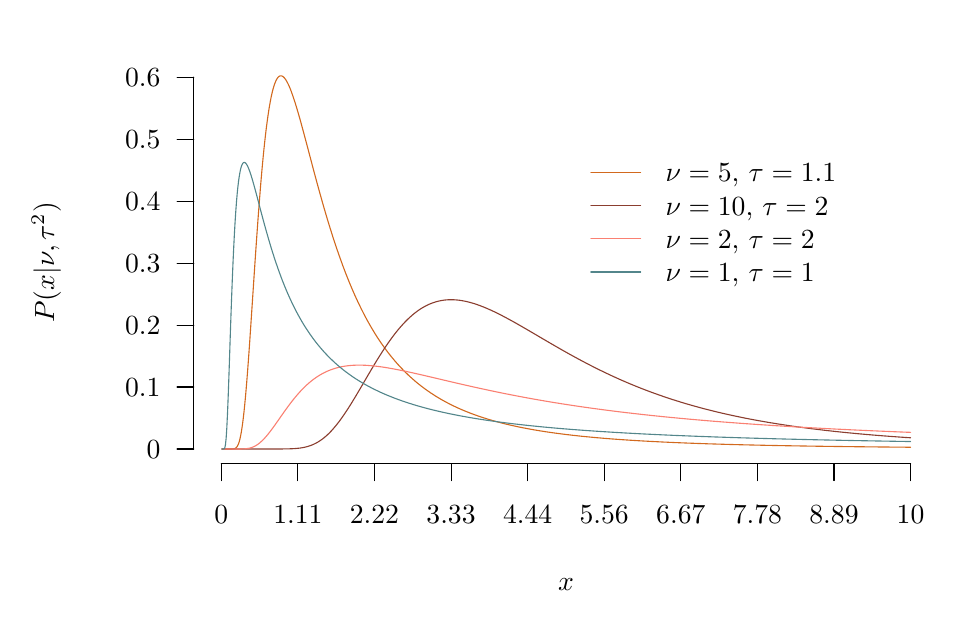
\begin{tikzpicture}[x=1pt,y=1pt]
\definecolor{fillColor}{RGB}{255,255,255}
\path[use as bounding box,fill=fillColor,fill opacity=0.00] (0,0) rectangle (329.00,205.63);
\begin{scope}
\path[clip] ( 60.00, 48.00) rectangle (329.00,193.63);
\definecolor{drawColor}{RGB}{210,105,30}

\path[draw=drawColor,line width= 0.4pt,line join=round,line cap=round] ( 70.21, 53.39) --
	( 70.46, 53.39) --
	( 70.71, 53.39) --
	( 70.96, 53.39) --
	( 71.21, 53.39) --
	( 71.46, 53.39) --
	( 71.71, 53.39) --
	( 71.96, 53.39) --
	( 72.21, 53.39) --
	( 72.46, 53.39) --
	( 72.71, 53.39) --
	( 72.96, 53.39) --
	( 73.20, 53.39) --
	( 73.45, 53.39) --
	( 73.70, 53.40) --
	( 73.95, 53.40) --
	( 74.20, 53.42) --
	( 74.45, 53.45) --
	( 74.70, 53.50) --
	( 74.95, 53.60) --
	( 75.20, 53.75) --
	( 75.45, 53.97) --
	( 75.70, 54.29) --
	( 75.95, 54.73) --
	( 76.20, 55.32) --
	( 76.45, 56.06) --
	( 76.70, 56.99) --
	( 76.94, 58.12) --
	( 77.19, 59.46) --
	( 77.44, 61.01) --
	( 77.69, 62.80) --
	( 77.94, 64.80) --
	( 78.19, 67.03) --
	( 78.44, 69.48) --
	( 78.69, 72.13) --
	( 78.94, 74.97) --
	( 79.19, 77.99) --
	( 79.44, 81.17) --
	( 79.69, 84.49) --
	( 79.94, 87.94) --
	( 80.19, 91.49) --
	( 80.43, 95.12) --
	( 80.68, 98.82) --
	( 80.93,102.57) --
	( 81.18,106.35) --
	( 81.43,110.13) --
	( 81.68,113.91) --
	( 81.93,117.67) --
	( 82.18,121.40) --
	( 82.43,125.07) --
	( 82.68,128.69) --
	( 82.93,132.23) --
	( 83.18,135.69) --
	( 83.43,139.07) --
	( 83.68,142.34) --
	( 83.93,145.52) --
	( 84.17,148.58) --
	( 84.42,151.53) --
	( 84.67,154.37) --
	( 84.92,157.08) --
	( 85.17,159.68) --
	( 85.42,162.15) --
	( 85.67,164.50) --
	( 85.92,166.72) --
	( 86.17,168.83) --
	( 86.42,170.81) --
	( 86.67,172.66) --
	( 86.92,174.40) --
	( 87.17,176.03) --
	( 87.42,177.53) --
	( 87.67,178.92) --
	( 87.91,180.21) --
	( 88.16,181.38) --
	( 88.41,182.45) --
	( 88.66,183.42) --
	( 88.91,184.29) --
	( 89.16,185.06) --
	( 89.41,185.74) --
	( 89.66,186.33) --
	( 89.91,186.84) --
	( 90.16,187.26) --
	( 90.41,187.60) --
	( 90.66,187.87) --
	( 90.91,188.06) --
	( 91.16,188.18) --
	( 91.41,188.23) --
	( 91.65,188.22) --
	( 91.90,188.15) --
	( 92.15,188.02) --
	( 92.40,187.84) --
	( 92.65,187.60) --
	( 92.90,187.31) --
	( 93.15,186.97) --
	( 93.40,186.59) --
	( 93.65,186.17) --
	( 93.90,185.70) --
	( 94.15,185.20) --
	( 94.40,184.66) --
	( 94.65,184.08) --
	( 94.90,183.48) --
	( 95.15,182.84) --
	( 95.39,182.17) --
	( 95.64,181.48) --
	( 95.89,180.77) --
	( 96.14,180.03) --
	( 96.39,179.27) --
	( 96.64,178.49) --
	( 96.89,177.69) --
	( 97.14,176.87) --
	( 97.39,176.04) --
	( 97.64,175.19) --
	( 97.89,174.33) --
	( 98.14,173.46) --
	( 98.39,172.58) --
	( 98.64,171.69) --
	( 98.89,170.79) --
	( 99.13,169.88) --
	( 99.38,168.96) --
	( 99.63,168.04) --
	( 99.88,167.11) --
	(100.13,166.18) --
	(100.38,165.24) --
	(100.63,164.30) --
	(100.88,163.36) --
	(101.13,162.42) --
	(101.38,161.47) --
	(101.63,160.53) --
	(101.88,159.58) --
	(102.13,158.64) --
	(102.38,157.69) --
	(102.63,156.75) --
	(102.87,155.81) --
	(103.12,154.87) --
	(103.37,153.94) --
	(103.62,153.00) --
	(103.87,152.08) --
	(104.12,151.15) --
	(104.37,150.23) --
	(104.62,149.31) --
	(104.87,148.40) --
	(105.12,147.49) --
	(105.37,146.59) --
	(105.62,145.69) --
	(105.87,144.80) --
	(106.12,143.91) --
	(106.37,143.03) --
	(106.61,142.16) --
	(106.86,141.29) --
	(107.11,140.42) --
	(107.36,139.57) --
	(107.61,138.72) --
	(107.86,137.87) --
	(108.11,137.04) --
	(108.36,136.21) --
	(108.61,135.38) --
	(108.86,134.57) --
	(109.11,133.76) --
	(109.36,132.95) --
	(109.61,132.16) --
	(109.86,131.37) --
	(110.10,130.59) --
	(110.35,129.81) --
	(110.60,129.05) --
	(110.85,128.28) --
	(111.10,127.53) --
	(111.35,126.79) --
	(111.60,126.05) --
	(111.85,125.31) --
	(112.10,124.59) --
	(112.35,123.87) --
	(112.60,123.16) --
	(112.85,122.46) --
	(113.10,121.76) --
	(113.35,121.07) --
	(113.60,120.39) --
	(113.84,119.71) --
	(114.09,119.05) --
	(114.34,118.39) --
	(114.59,117.73) --
	(114.84,117.08) --
	(115.09,116.44) --
	(115.34,115.81) --
	(115.59,115.18) --
	(115.84,114.56) --
	(116.09,113.94) --
	(116.34,113.34) --
	(116.59,112.74) --
	(116.84,112.14) --
	(117.09,111.55) --
	(117.34,110.97) --
	(117.58,110.40) --
	(117.83,109.83) --
	(118.08,109.26) --
	(118.33,108.71) --
	(118.58,108.16) --
	(118.83,107.61) --
	(119.08,107.07) --
	(119.33,106.54) --
	(119.58,106.01) --
	(119.83,105.49) --
	(120.08,104.98) --
	(120.33,104.47) --
	(120.58,103.96) --
	(120.83,103.47) --
	(121.08,102.97) --
	(121.32,102.49) --
	(121.57,102.00) --
	(121.82,101.53) --
	(122.07,101.06) --
	(122.32,100.59) --
	(122.57,100.13) --
	(122.82, 99.67) --
	(123.07, 99.22) --
	(123.32, 98.78) --
	(123.57, 98.34) --
	(123.82, 97.90) --
	(124.07, 97.47) --
	(124.32, 97.05) --
	(124.57, 96.63) --
	(124.82, 96.21) --
	(125.06, 95.80) --
	(125.31, 95.39) --
	(125.56, 94.99) --
	(125.81, 94.59) --
	(126.06, 94.20) --
	(126.31, 93.81) --
	(126.56, 93.42) --
	(126.81, 93.04) --
	(127.06, 92.67) --
	(127.31, 92.30) --
	(127.56, 91.93) --
	(127.81, 91.56) --
	(128.06, 91.21) --
	(128.31, 90.85) --
	(128.56, 90.50) --
	(128.80, 90.15) --
	(129.05, 89.81) --
	(129.30, 89.47) --
	(129.55, 89.13) --
	(129.80, 88.80) --
	(130.05, 88.47) --
	(130.30, 88.14) --
	(130.55, 87.82) --
	(130.80, 87.51) --
	(131.05, 87.19) --
	(131.30, 86.88) --
	(131.55, 86.57) --
	(131.80, 86.27) --
	(132.05, 85.97) --
	(132.30, 85.67) --
	(132.54, 85.38) --
	(132.79, 85.08) --
	(133.04, 84.80) --
	(133.29, 84.51) --
	(133.54, 84.23) --
	(133.79, 83.95) --
	(134.04, 83.68) --
	(134.29, 83.40) --
	(134.54, 83.14) --
	(134.79, 82.87) --
	(135.04, 82.61) --
	(135.29, 82.34) --
	(135.54, 82.09) --
	(135.79, 81.83) --
	(136.04, 81.58) --
	(136.28, 81.33) --
	(136.53, 81.08) --
	(136.78, 80.84) --
	(137.03, 80.60) --
	(137.28, 80.36) --
	(137.53, 80.12) --
	(137.78, 79.89) --
	(138.03, 79.66) --
	(138.28, 79.43) --
	(138.53, 79.20) --
	(138.78, 78.98) --
	(139.03, 78.75) --
	(139.28, 78.54) --
	(139.53, 78.32) --
	(139.77, 78.10) --
	(140.02, 77.89) --
	(140.27, 77.68) --
	(140.52, 77.47) --
	(140.77, 77.27) --
	(141.02, 77.06) --
	(141.27, 76.86) --
	(141.52, 76.66) --
	(141.77, 76.46) --
	(142.02, 76.27) --
	(142.27, 76.08) --
	(142.52, 75.88) --
	(142.77, 75.70) --
	(143.02, 75.51) --
	(143.27, 75.32) --
	(143.51, 75.14) --
	(143.76, 74.96) --
	(144.01, 74.78) --
	(144.26, 74.60) --
	(144.51, 74.42) --
	(144.76, 74.25) --
	(145.01, 74.08) --
	(145.26, 73.91) --
	(145.51, 73.74) --
	(145.76, 73.57) --
	(146.01, 73.41) --
	(146.26, 73.24) --
	(146.51, 73.08) --
	(146.76, 72.92) --
	(147.01, 72.76) --
	(147.25, 72.60) --
	(147.50, 72.45) --
	(147.75, 72.29) --
	(148.00, 72.14) --
	(148.25, 71.99) --
	(148.50, 71.84) --
	(148.75, 71.69) --
	(149.00, 71.55) --
	(149.25, 71.40) --
	(149.50, 71.26) --
	(149.75, 71.11) --
	(150.00, 70.97) --
	(150.25, 70.83) --
	(150.50, 70.70) --
	(150.75, 70.56) --
	(150.99, 70.42) --
	(151.24, 70.29) --
	(151.49, 70.16) --
	(151.74, 70.03) --
	(151.99, 69.90) --
	(152.24, 69.77) --
	(152.49, 69.64) --
	(152.74, 69.51) --
	(152.99, 69.39) --
	(153.24, 69.26) --
	(153.49, 69.14) --
	(153.74, 69.02) --
	(153.99, 68.90) --
	(154.24, 68.78) --
	(154.49, 68.66) --
	(154.73, 68.55) --
	(154.98, 68.43) --
	(155.23, 68.31) --
	(155.48, 68.20) --
	(155.73, 68.09) --
	(155.98, 67.98) --
	(156.23, 67.87) --
	(156.48, 67.76) --
	(156.73, 67.65) --
	(156.98, 67.54) --
	(157.23, 67.44) --
	(157.48, 67.33) --
	(157.73, 67.23) --
	(157.98, 67.12) --
	(158.23, 67.02) --
	(158.47, 66.92) --
	(158.72, 66.82) --
	(158.97, 66.72) --
	(159.22, 66.62) --
	(159.47, 66.52) --
	(159.72, 66.43) --
	(159.97, 66.33) --
	(160.22, 66.24) --
	(160.47, 66.14) --
	(160.72, 66.05) --
	(160.97, 65.96) --
	(161.22, 65.86) --
	(161.47, 65.77) --
	(161.72, 65.68) --
	(161.97, 65.59) --
	(162.21, 65.51) --
	(162.46, 65.42) --
	(162.71, 65.33) --
	(162.96, 65.25) --
	(163.21, 65.16) --
	(163.46, 65.08) --
	(163.71, 64.99) --
	(163.96, 64.91) --
	(164.21, 64.83) --
	(164.46, 64.75) --
	(164.71, 64.67) --
	(164.96, 64.59) --
	(165.21, 64.51) --
	(165.46, 64.43) --
	(165.71, 64.35) --
	(165.95, 64.27) --
	(166.20, 64.20) --
	(166.45, 64.12) --
	(166.70, 64.05) --
	(166.95, 63.97) --
	(167.20, 63.90) --
	(167.45, 63.83) --
	(167.70, 63.75) --
	(167.95, 63.68) --
	(168.20, 63.61) --
	(168.45, 63.54) --
	(168.70, 63.47) --
	(168.95, 63.40) --
	(169.20, 63.33) --
	(169.45, 63.26) --
	(169.69, 63.20) --
	(169.94, 63.13) --
	(170.19, 63.06) --
	(170.44, 63.00) --
	(170.69, 62.93) --
	(170.94, 62.87) --
	(171.19, 62.80) --
	(171.44, 62.74) --
	(171.69, 62.68) --
	(171.94, 62.61) --
	(172.19, 62.55) --
	(172.44, 62.49) --
	(172.69, 62.43) --
	(172.94, 62.37) --
	(173.18, 62.31) --
	(173.43, 62.25) --
	(173.68, 62.19) --
	(173.93, 62.13) --
	(174.18, 62.07) --
	(174.43, 62.02) --
	(174.68, 61.96) --
	(174.93, 61.90) --
	(175.18, 61.85) --
	(175.43, 61.79) --
	(175.68, 61.74) --
	(175.93, 61.68) --
	(176.18, 61.63) --
	(176.43, 61.57) --
	(176.68, 61.52) --
	(176.92, 61.47) --
	(177.17, 61.42) --
	(177.42, 61.36) --
	(177.67, 61.31) --
	(177.92, 61.26) --
	(178.17, 61.21) --
	(178.42, 61.16) --
	(178.67, 61.11) --
	(178.92, 61.06) --
	(179.17, 61.01) --
	(179.42, 60.96) --
	(179.67, 60.91) --
	(179.92, 60.87) --
	(180.17, 60.82) --
	(180.42, 60.77) --
	(180.66, 60.73) --
	(180.91, 60.68) --
	(181.16, 60.63) --
	(181.41, 60.59) --
	(181.66, 60.54) --
	(181.91, 60.50) --
	(182.16, 60.45) --
	(182.41, 60.41) --
	(182.66, 60.36) --
	(182.91, 60.32) --
	(183.16, 60.28) --
	(183.41, 60.24) --
	(183.66, 60.19) --
	(183.91, 60.15) --
	(184.16, 60.11) --
	(184.40, 60.07) --
	(184.65, 60.03) --
	(184.90, 59.99) --
	(185.15, 59.94) --
	(185.40, 59.90) --
	(185.65, 59.86) --
	(185.90, 59.83) --
	(186.15, 59.79) --
	(186.40, 59.75) --
	(186.65, 59.71) --
	(186.90, 59.67) --
	(187.15, 59.63) --
	(187.40, 59.59) --
	(187.65, 59.56) --
	(187.90, 59.52) --
	(188.14, 59.48) --
	(188.39, 59.45) --
	(188.64, 59.41) --
	(188.89, 59.37) --
	(189.14, 59.34) --
	(189.39, 59.30) --
	(189.64, 59.27) --
	(189.89, 59.23) --
	(190.14, 59.20) --
	(190.39, 59.16) --
	(190.64, 59.13) --
	(190.89, 59.09) --
	(191.14, 59.06) --
	(191.39, 59.03) --
	(191.64, 58.99) --
	(191.88, 58.96) --
	(192.13, 58.93) --
	(192.38, 58.90) --
	(192.63, 58.86) --
	(192.88, 58.83) --
	(193.13, 58.80) --
	(193.38, 58.77) --
	(193.63, 58.74) --
	(193.88, 58.71) --
	(194.13, 58.68) --
	(194.38, 58.65) --
	(194.63, 58.61) --
	(194.88, 58.58) --
	(195.13, 58.55) --
	(195.38, 58.53) --
	(195.62, 58.50) --
	(195.87, 58.47) --
	(196.12, 58.44) --
	(196.37, 58.41) --
	(196.62, 58.38) --
	(196.87, 58.35) --
	(197.12, 58.32) --
	(197.37, 58.30) --
	(197.62, 58.27) --
	(197.87, 58.24) --
	(198.12, 58.21) --
	(198.37, 58.19) --
	(198.62, 58.16) --
	(198.87, 58.13) --
	(199.12, 58.10) --
	(199.36, 58.08) --
	(199.61, 58.05) --
	(199.86, 58.03) --
	(200.11, 58.00) --
	(200.36, 57.97) --
	(200.61, 57.95) --
	(200.86, 57.92) --
	(201.11, 57.90) --
	(201.36, 57.87) --
	(201.61, 57.85) --
	(201.86, 57.82) --
	(202.11, 57.80) --
	(202.36, 57.78) --
	(202.61, 57.75) --
	(202.85, 57.73) --
	(203.10, 57.70) --
	(203.35, 57.68) --
	(203.60, 57.66) --
	(203.85, 57.63) --
	(204.10, 57.61) --
	(204.35, 57.59) --
	(204.60, 57.56) --
	(204.85, 57.54) --
	(205.10, 57.52) --
	(205.35, 57.50) --
	(205.60, 57.47) --
	(205.85, 57.45) --
	(206.10, 57.43) --
	(206.35, 57.41) --
	(206.59, 57.39) --
	(206.84, 57.37) --
	(207.09, 57.35) --
	(207.34, 57.32) --
	(207.59, 57.30) --
	(207.84, 57.28) --
	(208.09, 57.26) --
	(208.34, 57.24) --
	(208.59, 57.22) --
	(208.84, 57.20) --
	(209.09, 57.18) --
	(209.34, 57.16) --
	(209.59, 57.14) --
	(209.84, 57.12) --
	(210.09, 57.10) --
	(210.33, 57.08) --
	(210.58, 57.06) --
	(210.83, 57.04) --
	(211.08, 57.02) --
	(211.33, 57.00) --
	(211.58, 56.99) --
	(211.83, 56.97) --
	(212.08, 56.95) --
	(212.33, 56.93) --
	(212.58, 56.91) --
	(212.83, 56.89) --
	(213.08, 56.88) --
	(213.33, 56.86) --
	(213.58, 56.84) --
	(213.83, 56.82) --
	(214.07, 56.80) --
	(214.32, 56.79) --
	(214.57, 56.77) --
	(214.82, 56.75) --
	(215.07, 56.73) --
	(215.32, 56.72) --
	(215.57, 56.70) --
	(215.82, 56.68) --
	(216.07, 56.67) --
	(216.32, 56.65) --
	(216.57, 56.63) --
	(216.82, 56.62) --
	(217.07, 56.60) --
	(217.32, 56.59) --
	(217.57, 56.57) --
	(217.81, 56.55) --
	(218.06, 56.54) --
	(218.31, 56.52) --
	(218.56, 56.51) --
	(218.81, 56.49) --
	(219.06, 56.47) --
	(219.31, 56.46) --
	(219.56, 56.44) --
	(219.81, 56.43) --
	(220.06, 56.41) --
	(220.31, 56.40) --
	(220.56, 56.38) --
	(220.81, 56.37) --
	(221.06, 56.35) --
	(221.31, 56.34) --
	(221.55, 56.33) --
	(221.80, 56.31) --
	(222.05, 56.30) --
	(222.30, 56.28) --
	(222.55, 56.27) --
	(222.80, 56.25) --
	(223.05, 56.24) --
	(223.30, 56.23) --
	(223.55, 56.21) --
	(223.80, 56.20) --
	(224.05, 56.19) --
	(224.30, 56.17) --
	(224.55, 56.16) --
	(224.80, 56.14) --
	(225.05, 56.13) --
	(225.29, 56.12) --
	(225.54, 56.10) --
	(225.79, 56.09) --
	(226.04, 56.08) --
	(226.29, 56.07) --
	(226.54, 56.05) --
	(226.79, 56.04) --
	(227.04, 56.03) --
	(227.29, 56.02) --
	(227.54, 56.00) --
	(227.79, 55.99) --
	(228.04, 55.98) --
	(228.29, 55.97) --
	(228.54, 55.95) --
	(228.79, 55.94) --
	(229.03, 55.93) --
	(229.28, 55.92) --
	(229.53, 55.91) --
	(229.78, 55.89) --
	(230.03, 55.88) --
	(230.28, 55.87) --
	(230.53, 55.86) --
	(230.78, 55.85) --
	(231.03, 55.84) --
	(231.28, 55.82) --
	(231.53, 55.81) --
	(231.78, 55.80) --
	(232.03, 55.79) --
	(232.28, 55.78) --
	(232.53, 55.77) --
	(232.77, 55.76) --
	(233.02, 55.75) --
	(233.27, 55.73) --
	(233.52, 55.72) --
	(233.77, 55.71) --
	(234.02, 55.70) --
	(234.27, 55.69) --
	(234.52, 55.68) --
	(234.77, 55.67) --
	(235.02, 55.66) --
	(235.27, 55.65) --
	(235.52, 55.64) --
	(235.77, 55.63) --
	(236.02, 55.62) --
	(236.26, 55.61) --
	(236.51, 55.60) --
	(236.76, 55.59) --
	(237.01, 55.58) --
	(237.26, 55.57) --
	(237.51, 55.56) --
	(237.76, 55.55) --
	(238.01, 55.54) --
	(238.26, 55.53) --
	(238.51, 55.52) --
	(238.76, 55.51) --
	(239.01, 55.50) --
	(239.26, 55.49) --
	(239.51, 55.48) --
	(239.76, 55.47) --
	(240.00, 55.46) --
	(240.25, 55.45) --
	(240.50, 55.45) --
	(240.75, 55.44) --
	(241.00, 55.43) --
	(241.25, 55.42) --
	(241.50, 55.41) --
	(241.75, 55.40) --
	(242.00, 55.39) --
	(242.25, 55.38) --
	(242.50, 55.37) --
	(242.75, 55.36) --
	(243.00, 55.36) --
	(243.25, 55.35) --
	(243.50, 55.34) --
	(243.74, 55.33) --
	(243.99, 55.32) --
	(244.24, 55.31) --
	(244.49, 55.30) --
	(244.74, 55.30) --
	(244.99, 55.29) --
	(245.24, 55.28) --
	(245.49, 55.27) --
	(245.74, 55.26) --
	(245.99, 55.26) --
	(246.24, 55.25) --
	(246.49, 55.24) --
	(246.74, 55.23) --
	(246.99, 55.22) --
	(247.24, 55.22) --
	(247.48, 55.21) --
	(247.73, 55.20) --
	(247.98, 55.19) --
	(248.23, 55.18) --
	(248.48, 55.18) --
	(248.73, 55.17) --
	(248.98, 55.16) --
	(249.23, 55.15) --
	(249.48, 55.15) --
	(249.73, 55.14) --
	(249.98, 55.13) --
	(250.23, 55.12) --
	(250.48, 55.12) --
	(250.73, 55.11) --
	(250.98, 55.10) --
	(251.22, 55.09) --
	(251.47, 55.09) --
	(251.72, 55.08) --
	(251.97, 55.07) --
	(252.22, 55.07) --
	(252.47, 55.06) --
	(252.72, 55.05) --
	(252.97, 55.05) --
	(253.22, 55.04) --
	(253.47, 55.03) --
	(253.72, 55.02) --
	(253.97, 55.02) --
	(254.22, 55.01) --
	(254.47, 55.00) --
	(254.72, 55.00) --
	(254.96, 54.99) --
	(255.21, 54.98) --
	(255.46, 54.98) --
	(255.71, 54.97) --
	(255.96, 54.96) --
	(256.21, 54.96) --
	(256.46, 54.95) --
	(256.71, 54.95) --
	(256.96, 54.94) --
	(257.21, 54.93) --
	(257.46, 54.93) --
	(257.71, 54.92) --
	(257.96, 54.91) --
	(258.21, 54.91) --
	(258.46, 54.90) --
	(258.70, 54.89) --
	(258.95, 54.89) --
	(259.20, 54.88) --
	(259.45, 54.88) --
	(259.70, 54.87) --
	(259.95, 54.86) --
	(260.20, 54.86) --
	(260.45, 54.85) --
	(260.70, 54.85) --
	(260.95, 54.84) --
	(261.20, 54.83) --
	(261.45, 54.83) --
	(261.70, 54.82) --
	(261.95, 54.82) --
	(262.20, 54.81) --
	(262.44, 54.81) --
	(262.69, 54.80) --
	(262.94, 54.79) --
	(263.19, 54.79) --
	(263.44, 54.78) --
	(263.69, 54.78) --
	(263.94, 54.77) --
	(264.19, 54.77) --
	(264.44, 54.76) --
	(264.69, 54.76) --
	(264.94, 54.75) --
	(265.19, 54.75) --
	(265.44, 54.74) --
	(265.69, 54.73) --
	(265.93, 54.73) --
	(266.18, 54.72) --
	(266.43, 54.72) --
	(266.68, 54.71) --
	(266.93, 54.71) --
	(267.18, 54.70) --
	(267.43, 54.70) --
	(267.68, 54.69) --
	(267.93, 54.69) --
	(268.18, 54.68) --
	(268.43, 54.68) --
	(268.68, 54.67) --
	(268.93, 54.67) --
	(269.18, 54.66) --
	(269.43, 54.66) --
	(269.67, 54.65) --
	(269.92, 54.65) --
	(270.17, 54.64) --
	(270.42, 54.64) --
	(270.67, 54.63) --
	(270.92, 54.63) --
	(271.17, 54.62) --
	(271.42, 54.62) --
	(271.67, 54.61) --
	(271.92, 54.61) --
	(272.17, 54.60) --
	(272.42, 54.60) --
	(272.67, 54.60) --
	(272.92, 54.59) --
	(273.17, 54.59) --
	(273.41, 54.58) --
	(273.66, 54.58) --
	(273.91, 54.57) --
	(274.16, 54.57) --
	(274.41, 54.56) --
	(274.66, 54.56) --
	(274.91, 54.55) --
	(275.16, 54.55) --
	(275.41, 54.55) --
	(275.66, 54.54) --
	(275.91, 54.54) --
	(276.16, 54.53) --
	(276.41, 54.53) --
	(276.66, 54.52) --
	(276.91, 54.52) --
	(277.15, 54.52) --
	(277.40, 54.51) --
	(277.65, 54.51) --
	(277.90, 54.50) --
	(278.15, 54.50) --
	(278.40, 54.50) --
	(278.65, 54.49) --
	(278.90, 54.49) --
	(279.15, 54.48) --
	(279.40, 54.48) --
	(279.65, 54.47) --
	(279.90, 54.47) --
	(280.15, 54.47) --
	(280.40, 54.46) --
	(280.65, 54.46) --
	(280.89, 54.45) --
	(281.14, 54.45) --
	(281.39, 54.45) --
	(281.64, 54.44) --
	(281.89, 54.44) --
	(282.14, 54.44) --
	(282.39, 54.43) --
	(282.64, 54.43) --
	(282.89, 54.42) --
	(283.14, 54.42) --
	(283.39, 54.42) --
	(283.64, 54.41) --
	(283.89, 54.41) --
	(284.14, 54.40) --
	(284.39, 54.40) --
	(284.63, 54.40) --
	(284.88, 54.39) --
	(285.13, 54.39) --
	(285.38, 54.39) --
	(285.63, 54.38) --
	(285.88, 54.38) --
	(286.13, 54.38) --
	(286.38, 54.37) --
	(286.63, 54.37) --
	(286.88, 54.37) --
	(287.13, 54.36) --
	(287.38, 54.36) --
	(287.63, 54.35) --
	(287.88, 54.35) --
	(288.13, 54.35) --
	(288.37, 54.34) --
	(288.62, 54.34) --
	(288.87, 54.34) --
	(289.12, 54.33) --
	(289.37, 54.33) --
	(289.62, 54.33) --
	(289.87, 54.32) --
	(290.12, 54.32) --
	(290.37, 54.32) --
	(290.62, 54.31) --
	(290.87, 54.31) --
	(291.12, 54.31) --
	(291.37, 54.30) --
	(291.62, 54.30) --
	(291.87, 54.30) --
	(292.11, 54.29) --
	(292.36, 54.29) --
	(292.61, 54.29) --
	(292.86, 54.29) --
	(293.11, 54.28) --
	(293.36, 54.28) --
	(293.61, 54.28) --
	(293.86, 54.27) --
	(294.11, 54.27) --
	(294.36, 54.27) --
	(294.61, 54.26) --
	(294.86, 54.26) --
	(295.11, 54.26) --
	(295.36, 54.25) --
	(295.61, 54.25) --
	(295.85, 54.25) --
	(296.10, 54.25) --
	(296.35, 54.24) --
	(296.60, 54.24) --
	(296.85, 54.24) --
	(297.10, 54.23) --
	(297.35, 54.23) --
	(297.60, 54.23) --
	(297.85, 54.22) --
	(298.10, 54.22) --
	(298.35, 54.22) --
	(298.60, 54.22) --
	(298.85, 54.21) --
	(299.10, 54.21) --
	(299.34, 54.21) --
	(299.59, 54.21) --
	(299.84, 54.20) --
	(300.09, 54.20) --
	(300.34, 54.20) --
	(300.59, 54.19) --
	(300.84, 54.19) --
	(301.09, 54.19) --
	(301.34, 54.19) --
	(301.59, 54.18) --
	(301.84, 54.18) --
	(302.09, 54.18) --
	(302.34, 54.18) --
	(302.59, 54.17) --
	(302.84, 54.17) --
	(303.08, 54.17) --
	(303.33, 54.16) --
	(303.58, 54.16) --
	(303.83, 54.16) --
	(304.08, 54.16) --
	(304.33, 54.15) --
	(304.58, 54.15) --
	(304.83, 54.15) --
	(305.08, 54.15) --
	(305.33, 54.14) --
	(305.58, 54.14) --
	(305.83, 54.14) --
	(306.08, 54.14) --
	(306.33, 54.13) --
	(306.58, 54.13) --
	(306.82, 54.13) --
	(307.07, 54.13) --
	(307.32, 54.12) --
	(307.57, 54.12) --
	(307.82, 54.12) --
	(308.07, 54.12) --
	(308.32, 54.11) --
	(308.57, 54.11) --
	(308.82, 54.11) --
	(309.07, 54.11) --
	(309.32, 54.10) --
	(309.57, 54.10) --
	(309.82, 54.10) --
	(310.07, 54.10) --
	(310.32, 54.10) --
	(310.56, 54.09) --
	(310.81, 54.09) --
	(311.06, 54.09) --
	(311.31, 54.09) --
	(311.56, 54.08) --
	(311.81, 54.08) --
	(312.06, 54.08) --
	(312.31, 54.08) --
	(312.56, 54.07) --
	(312.81, 54.07) --
	(313.06, 54.07) --
	(313.31, 54.07) --
	(313.56, 54.07) --
	(313.81, 54.06) --
	(314.06, 54.06) --
	(314.30, 54.06) --
	(314.55, 54.06) --
	(314.80, 54.06) --
	(315.05, 54.05) --
	(315.30, 54.05) --
	(315.55, 54.05) --
	(315.80, 54.05) --
	(316.05, 54.04) --
	(316.30, 54.04) --
	(316.55, 54.04) --
	(316.80, 54.04) --
	(317.05, 54.04) --
	(317.30, 54.03) --
	(317.55, 54.03) --
	(317.80, 54.03) --
	(318.04, 54.03) --
	(318.29, 54.03) --
	(318.54, 54.02) --
	(318.79, 54.02) --
	(319.04, 54.02);
\end{scope}
\begin{scope}
\path[clip] ( 60.00, 48.00) rectangle (329.00,193.63);
\definecolor{drawColor}{RGB}{139,62,47}

\path[draw=drawColor,line width= 0.4pt,line join=round,line cap=round] ( 70.21, 53.39) --
	( 70.46, 53.39) --
	( 70.71, 53.39) --
	( 70.96, 53.39) --
	( 71.21, 53.39) --
	( 71.46, 53.39) --
	( 71.71, 53.39) --
	( 71.96, 53.39) --
	( 72.21, 53.39) --
	( 72.46, 53.39) --
	( 72.71, 53.39) --
	( 72.96, 53.39) --
	( 73.20, 53.39) --
	( 73.45, 53.39) --
	( 73.70, 53.39) --
	( 73.95, 53.39) --
	( 74.20, 53.39) --
	( 74.45, 53.39) --
	( 74.70, 53.39) --
	( 74.95, 53.39) --
	( 75.20, 53.39) --
	( 75.45, 53.39) --
	( 75.70, 53.39) --
	( 75.95, 53.39) --
	( 76.20, 53.39) --
	( 76.45, 53.39) --
	( 76.70, 53.39) --
	( 76.94, 53.39) --
	( 77.19, 53.39) --
	( 77.44, 53.39) --
	( 77.69, 53.39) --
	( 77.94, 53.39) --
	( 78.19, 53.39) --
	( 78.44, 53.39) --
	( 78.69, 53.39) --
	( 78.94, 53.39) --
	( 79.19, 53.39) --
	( 79.44, 53.39) --
	( 79.69, 53.39) --
	( 79.94, 53.39) --
	( 80.19, 53.39) --
	( 80.43, 53.39) --
	( 80.68, 53.39) --
	( 80.93, 53.39) --
	( 81.18, 53.39) --
	( 81.43, 53.39) --
	( 81.68, 53.39) --
	( 81.93, 53.39) --
	( 82.18, 53.39) --
	( 82.43, 53.39) --
	( 82.68, 53.39) --
	( 82.93, 53.39) --
	( 83.18, 53.39) --
	( 83.43, 53.39) --
	( 83.68, 53.39) --
	( 83.93, 53.39) --
	( 84.17, 53.39) --
	( 84.42, 53.39) --
	( 84.67, 53.39) --
	( 84.92, 53.39) --
	( 85.17, 53.39) --
	( 85.42, 53.39) --
	( 85.67, 53.39) --
	( 85.92, 53.39) --
	( 86.17, 53.39) --
	( 86.42, 53.39) --
	( 86.67, 53.39) --
	( 86.92, 53.39) --
	( 87.17, 53.39) --
	( 87.42, 53.39) --
	( 87.67, 53.39) --
	( 87.91, 53.39) --
	( 88.16, 53.39) --
	( 88.41, 53.39) --
	( 88.66, 53.39) --
	( 88.91, 53.39) --
	( 89.16, 53.39) --
	( 89.41, 53.39) --
	( 89.66, 53.39) --
	( 89.91, 53.40) --
	( 90.16, 53.40) --
	( 90.41, 53.40) --
	( 90.66, 53.40) --
	( 90.91, 53.40) --
	( 91.16, 53.40) --
	( 91.41, 53.40) --
	( 91.65, 53.40) --
	( 91.90, 53.40) --
	( 92.15, 53.40) --
	( 92.40, 53.41) --
	( 92.65, 53.41) --
	( 92.90, 53.41) --
	( 93.15, 53.42) --
	( 93.40, 53.42) --
	( 93.65, 53.42) --
	( 93.90, 53.43) --
	( 94.15, 53.43) --
	( 94.40, 53.44) --
	( 94.65, 53.45) --
	( 94.90, 53.46) --
	( 95.15, 53.47) --
	( 95.39, 53.48) --
	( 95.64, 53.49) --
	( 95.89, 53.50) --
	( 96.14, 53.51) --
	( 96.39, 53.53) --
	( 96.64, 53.55) --
	( 96.89, 53.57) --
	( 97.14, 53.59) --
	( 97.39, 53.61) --
	( 97.64, 53.64) --
	( 97.89, 53.66) --
	( 98.14, 53.69) --
	( 98.39, 53.72) --
	( 98.64, 53.76) --
	( 98.89, 53.80) --
	( 99.13, 53.84) --
	( 99.38, 53.88) --
	( 99.63, 53.93) --
	( 99.88, 53.98) --
	(100.13, 54.03) --
	(100.38, 54.09) --
	(100.63, 54.15) --
	(100.88, 54.21) --
	(101.13, 54.28) --
	(101.38, 54.36) --
	(101.63, 54.43) --
	(101.88, 54.52) --
	(102.13, 54.60) --
	(102.38, 54.69) --
	(102.63, 54.79) --
	(102.87, 54.89) --
	(103.12, 55.00) --
	(103.37, 55.11) --
	(103.62, 55.22) --
	(103.87, 55.35) --
	(104.12, 55.47) --
	(104.37, 55.61) --
	(104.62, 55.75) --
	(104.87, 55.89) --
	(105.12, 56.04) --
	(105.37, 56.20) --
	(105.62, 56.36) --
	(105.87, 56.53) --
	(106.12, 56.70) --
	(106.37, 56.88) --
	(106.61, 57.07) --
	(106.86, 57.26) --
	(107.11, 57.46) --
	(107.36, 57.67) --
	(107.61, 57.88) --
	(107.86, 58.10) --
	(108.11, 58.32) --
	(108.36, 58.55) --
	(108.61, 58.79) --
	(108.86, 59.03) --
	(109.11, 59.28) --
	(109.36, 59.54) --
	(109.61, 59.80) --
	(109.86, 60.07) --
	(110.10, 60.34) --
	(110.35, 60.62) --
	(110.60, 60.91) --
	(110.85, 61.20) --
	(111.10, 61.49) --
	(111.35, 61.80) --
	(111.60, 62.11) --
	(111.85, 62.42) --
	(112.10, 62.74) --
	(112.35, 63.06) --
	(112.60, 63.39) --
	(112.85, 63.73) --
	(113.10, 64.07) --
	(113.35, 64.41) --
	(113.60, 64.76) --
	(113.84, 65.12) --
	(114.09, 65.47) --
	(114.34, 65.84) --
	(114.59, 66.21) --
	(114.84, 66.58) --
	(115.09, 66.95) --
	(115.34, 67.33) --
	(115.59, 67.71) --
	(115.84, 68.10) --
	(116.09, 68.49) --
	(116.34, 68.88) --
	(116.59, 69.28) --
	(116.84, 69.68) --
	(117.09, 70.08) --
	(117.34, 70.49) --
	(117.58, 70.90) --
	(117.83, 71.31) --
	(118.08, 71.72) --
	(118.33, 72.13) --
	(118.58, 72.55) --
	(118.83, 72.97) --
	(119.08, 73.39) --
	(119.33, 73.81) --
	(119.58, 74.23) --
	(119.83, 74.65) --
	(120.08, 75.08) --
	(120.33, 75.50) --
	(120.58, 75.93) --
	(120.83, 76.36) --
	(121.08, 76.78) --
	(121.32, 77.21) --
	(121.57, 77.64) --
	(121.82, 78.07) --
	(122.07, 78.49) --
	(122.32, 78.92) --
	(122.57, 79.35) --
	(122.82, 79.77) --
	(123.07, 80.20) --
	(123.32, 80.62) --
	(123.57, 81.05) --
	(123.82, 81.47) --
	(124.07, 81.89) --
	(124.32, 82.31) --
	(124.57, 82.73) --
	(124.82, 83.15) --
	(125.06, 83.57) --
	(125.31, 83.98) --
	(125.56, 84.39) --
	(125.81, 84.80) --
	(126.06, 85.21) --
	(126.31, 85.62) --
	(126.56, 86.02) --
	(126.81, 86.42) --
	(127.06, 86.82) --
	(127.31, 87.22) --
	(127.56, 87.61) --
	(127.81, 88.00) --
	(128.06, 88.39) --
	(128.31, 88.78) --
	(128.56, 89.16) --
	(128.80, 89.54) --
	(129.05, 89.92) --
	(129.30, 90.29) --
	(129.55, 90.66) --
	(129.80, 91.03) --
	(130.05, 91.39) --
	(130.30, 91.75) --
	(130.55, 92.10) --
	(130.80, 92.46) --
	(131.05, 92.80) --
	(131.30, 93.15) --
	(131.55, 93.49) --
	(131.80, 93.83) --
	(132.05, 94.16) --
	(132.30, 94.49) --
	(132.54, 94.81) --
	(132.79, 95.14) --
	(133.04, 95.45) --
	(133.29, 95.77) --
	(133.54, 96.08) --
	(133.79, 96.38) --
	(134.04, 96.68) --
	(134.29, 96.98) --
	(134.54, 97.27) --
	(134.79, 97.56) --
	(135.04, 97.84) --
	(135.29, 98.12) --
	(135.54, 98.40) --
	(135.79, 98.67) --
	(136.04, 98.94) --
	(136.28, 99.20) --
	(136.53, 99.46) --
	(136.78, 99.71) --
	(137.03, 99.96) --
	(137.28,100.21) --
	(137.53,100.45) --
	(137.78,100.68) --
	(138.03,100.91) --
	(138.28,101.14) --
	(138.53,101.36) --
	(138.78,101.58) --
	(139.03,101.80) --
	(139.28,102.01) --
	(139.53,102.21) --
	(139.77,102.41) --
	(140.02,102.61) --
	(140.27,102.80) --
	(140.52,102.99) --
	(140.77,103.17) --
	(141.02,103.35) --
	(141.27,103.53) --
	(141.52,103.70) --
	(141.77,103.87) --
	(142.02,104.03) --
	(142.27,104.19) --
	(142.52,104.34) --
	(142.77,104.49) --
	(143.02,104.63) --
	(143.27,104.78) --
	(143.51,104.91) --
	(143.76,105.04) --
	(144.01,105.17) --
	(144.26,105.30) --
	(144.51,105.42) --
	(144.76,105.54) --
	(145.01,105.65) --
	(145.26,105.76) --
	(145.51,105.86) --
	(145.76,105.96) --
	(146.01,106.06) --
	(146.26,106.15) --
	(146.51,106.24) --
	(146.76,106.33) --
	(147.01,106.41) --
	(147.25,106.49) --
	(147.50,106.56) --
	(147.75,106.63) --
	(148.00,106.70) --
	(148.25,106.76) --
	(148.50,106.82) --
	(148.75,106.88) --
	(149.00,106.93) --
	(149.25,106.98) --
	(149.50,107.03) --
	(149.75,107.07) --
	(150.00,107.11) --
	(150.25,107.15) --
	(150.50,107.18) --
	(150.75,107.21) --
	(150.99,107.23) --
	(151.24,107.26) --
	(151.49,107.28) --
	(151.74,107.29) --
	(151.99,107.31) --
	(152.24,107.32) --
	(152.49,107.32) --
	(152.74,107.33) --
	(152.99,107.33) --
	(153.24,107.33) --
	(153.49,107.32) --
	(153.74,107.32) --
	(153.99,107.31) --
	(154.24,107.29) --
	(154.49,107.28) --
	(154.73,107.26) --
	(154.98,107.24) --
	(155.23,107.22) --
	(155.48,107.19) --
	(155.73,107.16) --
	(155.98,107.13) --
	(156.23,107.10) --
	(156.48,107.06) --
	(156.73,107.02) --
	(156.98,106.98) --
	(157.23,106.94) --
	(157.48,106.89) --
	(157.73,106.84) --
	(157.98,106.79) --
	(158.23,106.74) --
	(158.47,106.69) --
	(158.72,106.63) --
	(158.97,106.57) --
	(159.22,106.51) --
	(159.47,106.45) --
	(159.72,106.38) --
	(159.97,106.31) --
	(160.22,106.24) --
	(160.47,106.17) --
	(160.72,106.10) --
	(160.97,106.03) --
	(161.22,105.95) --
	(161.47,105.87) --
	(161.72,105.79) --
	(161.97,105.71) --
	(162.21,105.62) --
	(162.46,105.54) --
	(162.71,105.45) --
	(162.96,105.36) --
	(163.21,105.27) --
	(163.46,105.18) --
	(163.71,105.09) --
	(163.96,104.99) --
	(164.21,104.89) --
	(164.46,104.80) --
	(164.71,104.70) --
	(164.96,104.60) --
	(165.21,104.49) --
	(165.46,104.39) --
	(165.71,104.28) --
	(165.95,104.18) --
	(166.20,104.07) --
	(166.45,103.96) --
	(166.70,103.85) --
	(166.95,103.74) --
	(167.20,103.63) --
	(167.45,103.52) --
	(167.70,103.40) --
	(167.95,103.28) --
	(168.20,103.17) --
	(168.45,103.05) --
	(168.70,102.93) --
	(168.95,102.81) --
	(169.20,102.69) --
	(169.45,102.57) --
	(169.69,102.45) --
	(169.94,102.32) --
	(170.19,102.20) --
	(170.44,102.07) --
	(170.69,101.95) --
	(170.94,101.82) --
	(171.19,101.69) --
	(171.44,101.56) --
	(171.69,101.43) --
	(171.94,101.30) --
	(172.19,101.17) --
	(172.44,101.04) --
	(172.69,100.91) --
	(172.94,100.77) --
	(173.18,100.64) --
	(173.43,100.51) --
	(173.68,100.37) --
	(173.93,100.24) --
	(174.18,100.10) --
	(174.43, 99.96) --
	(174.68, 99.83) --
	(174.93, 99.69) --
	(175.18, 99.55) --
	(175.43, 99.41) --
	(175.68, 99.27) --
	(175.93, 99.13) --
	(176.18, 98.99) --
	(176.43, 98.85) --
	(176.68, 98.71) --
	(176.92, 98.57) --
	(177.17, 98.43) --
	(177.42, 98.29) --
	(177.67, 98.14) --
	(177.92, 98.00) --
	(178.17, 97.86) --
	(178.42, 97.72) --
	(178.67, 97.57) --
	(178.92, 97.43) --
	(179.17, 97.28) --
	(179.42, 97.14) --
	(179.67, 97.00) --
	(179.92, 96.85) --
	(180.17, 96.71) --
	(180.42, 96.56) --
	(180.66, 96.42) --
	(180.91, 96.27) --
	(181.16, 96.13) --
	(181.41, 95.98) --
	(181.66, 95.83) --
	(181.91, 95.69) --
	(182.16, 95.54) --
	(182.41, 95.40) --
	(182.66, 95.25) --
	(182.91, 95.10) --
	(183.16, 94.96) --
	(183.41, 94.81) --
	(183.66, 94.66) --
	(183.91, 94.52) --
	(184.16, 94.37) --
	(184.40, 94.22) --
	(184.65, 94.08) --
	(184.90, 93.93) --
	(185.15, 93.78) --
	(185.40, 93.64) --
	(185.65, 93.49) --
	(185.90, 93.35) --
	(186.15, 93.20) --
	(186.40, 93.05) --
	(186.65, 92.91) --
	(186.90, 92.76) --
	(187.15, 92.61) --
	(187.40, 92.47) --
	(187.65, 92.32) --
	(187.90, 92.18) --
	(188.14, 92.03) --
	(188.39, 91.89) --
	(188.64, 91.74) --
	(188.89, 91.60) --
	(189.14, 91.45) --
	(189.39, 91.31) --
	(189.64, 91.16) --
	(189.89, 91.02) --
	(190.14, 90.87) --
	(190.39, 90.73) --
	(190.64, 90.58) --
	(190.89, 90.44) --
	(191.14, 90.30) --
	(191.39, 90.15) --
	(191.64, 90.01) --
	(191.88, 89.87) --
	(192.13, 89.73) --
	(192.38, 89.58) --
	(192.63, 89.44) --
	(192.88, 89.30) --
	(193.13, 89.16) --
	(193.38, 89.02) --
	(193.63, 88.87) --
	(193.88, 88.73) --
	(194.13, 88.59) --
	(194.38, 88.45) --
	(194.63, 88.31) --
	(194.88, 88.17) --
	(195.13, 88.03) --
	(195.38, 87.89) --
	(195.62, 87.75) --
	(195.87, 87.62) --
	(196.12, 87.48) --
	(196.37, 87.34) --
	(196.62, 87.20) --
	(196.87, 87.06) --
	(197.12, 86.93) --
	(197.37, 86.79) --
	(197.62, 86.65) --
	(197.87, 86.52) --
	(198.12, 86.38) --
	(198.37, 86.25) --
	(198.62, 86.11) --
	(198.87, 85.98) --
	(199.12, 85.84) --
	(199.36, 85.71) --
	(199.61, 85.58) --
	(199.86, 85.44) --
	(200.11, 85.31) --
	(200.36, 85.18) --
	(200.61, 85.04) --
	(200.86, 84.91) --
	(201.11, 84.78) --
	(201.36, 84.65) --
	(201.61, 84.52) --
	(201.86, 84.39) --
	(202.11, 84.26) --
	(202.36, 84.13) --
	(202.61, 84.00) --
	(202.85, 83.87) --
	(203.10, 83.74) --
	(203.35, 83.61) --
	(203.60, 83.49) --
	(203.85, 83.36) --
	(204.10, 83.23) --
	(204.35, 83.10) --
	(204.60, 82.98) --
	(204.85, 82.85) --
	(205.10, 82.73) --
	(205.35, 82.60) --
	(205.60, 82.48) --
	(205.85, 82.35) --
	(206.10, 82.23) --
	(206.35, 82.11) --
	(206.59, 81.98) --
	(206.84, 81.86) --
	(207.09, 81.74) --
	(207.34, 81.62) --
	(207.59, 81.50) --
	(207.84, 81.37) --
	(208.09, 81.25) --
	(208.34, 81.13) --
	(208.59, 81.01) --
	(208.84, 80.89) --
	(209.09, 80.78) --
	(209.34, 80.66) --
	(209.59, 80.54) --
	(209.84, 80.42) --
	(210.09, 80.30) --
	(210.33, 80.19) --
	(210.58, 80.07) --
	(210.83, 79.95) --
	(211.08, 79.84) --
	(211.33, 79.72) --
	(211.58, 79.61) --
	(211.83, 79.49) --
	(212.08, 79.38) --
	(212.33, 79.27) --
	(212.58, 79.15) --
	(212.83, 79.04) --
	(213.08, 78.93) --
	(213.33, 78.82) --
	(213.58, 78.71) --
	(213.83, 78.59) --
	(214.07, 78.48) --
	(214.32, 78.37) --
	(214.57, 78.26) --
	(214.82, 78.15) --
	(215.07, 78.05) --
	(215.32, 77.94) --
	(215.57, 77.83) --
	(215.82, 77.72) --
	(216.07, 77.61) --
	(216.32, 77.51) --
	(216.57, 77.40) --
	(216.82, 77.29) --
	(217.07, 77.19) --
	(217.32, 77.08) --
	(217.57, 76.98) --
	(217.81, 76.87) --
	(218.06, 76.77) --
	(218.31, 76.67) --
	(218.56, 76.56) --
	(218.81, 76.46) --
	(219.06, 76.36) --
	(219.31, 76.26) --
	(219.56, 76.16) --
	(219.81, 76.05) --
	(220.06, 75.95) --
	(220.31, 75.85) --
	(220.56, 75.75) --
	(220.81, 75.65) --
	(221.06, 75.56) --
	(221.31, 75.46) --
	(221.55, 75.36) --
	(221.80, 75.26) --
	(222.05, 75.16) --
	(222.30, 75.07) --
	(222.55, 74.97) --
	(222.80, 74.87) --
	(223.05, 74.78) --
	(223.30, 74.68) --
	(223.55, 74.59) --
	(223.80, 74.49) --
	(224.05, 74.40) --
	(224.30, 74.30) --
	(224.55, 74.21) --
	(224.80, 74.12) --
	(225.05, 74.03) --
	(225.29, 73.93) --
	(225.54, 73.84) --
	(225.79, 73.75) --
	(226.04, 73.66) --
	(226.29, 73.57) --
	(226.54, 73.48) --
	(226.79, 73.39) --
	(227.04, 73.30) --
	(227.29, 73.21) --
	(227.54, 73.12) --
	(227.79, 73.03) --
	(228.04, 72.94) --
	(228.29, 72.86) --
	(228.54, 72.77) --
	(228.79, 72.68) --
	(229.03, 72.60) --
	(229.28, 72.51) --
	(229.53, 72.42) --
	(229.78, 72.34) --
	(230.03, 72.25) --
	(230.28, 72.17) --
	(230.53, 72.08) --
	(230.78, 72.00) --
	(231.03, 71.92) --
	(231.28, 71.83) --
	(231.53, 71.75) --
	(231.78, 71.67) --
	(232.03, 71.59) --
	(232.28, 71.50) --
	(232.53, 71.42) --
	(232.77, 71.34) --
	(233.02, 71.26) --
	(233.27, 71.18) --
	(233.52, 71.10) --
	(233.77, 71.02) --
	(234.02, 70.94) --
	(234.27, 70.86) --
	(234.52, 70.78) --
	(234.77, 70.71) --
	(235.02, 70.63) --
	(235.27, 70.55) --
	(235.52, 70.47) --
	(235.77, 70.40) --
	(236.02, 70.32) --
	(236.26, 70.24) --
	(236.51, 70.17) --
	(236.76, 70.09) --
	(237.01, 70.02) --
	(237.26, 69.94) --
	(237.51, 69.87) --
	(237.76, 69.80) --
	(238.01, 69.72) --
	(238.26, 69.65) --
	(238.51, 69.58) --
	(238.76, 69.50) --
	(239.01, 69.43) --
	(239.26, 69.36) --
	(239.51, 69.29) --
	(239.76, 69.22) --
	(240.00, 69.14) --
	(240.25, 69.07) --
	(240.50, 69.00) --
	(240.75, 68.93) --
	(241.00, 68.86) --
	(241.25, 68.79) --
	(241.50, 68.72) --
	(241.75, 68.66) --
	(242.00, 68.59) --
	(242.25, 68.52) --
	(242.50, 68.45) --
	(242.75, 68.38) --
	(243.00, 68.32) --
	(243.25, 68.25) --
	(243.50, 68.18) --
	(243.74, 68.12) --
	(243.99, 68.05) --
	(244.24, 67.98) --
	(244.49, 67.92) --
	(244.74, 67.85) --
	(244.99, 67.79) --
	(245.24, 67.72) --
	(245.49, 67.66) --
	(245.74, 67.60) --
	(245.99, 67.53) --
	(246.24, 67.47) --
	(246.49, 67.41) --
	(246.74, 67.34) --
	(246.99, 67.28) --
	(247.24, 67.22) --
	(247.48, 67.16) --
	(247.73, 67.10) --
	(247.98, 67.03) --
	(248.23, 66.97) --
	(248.48, 66.91) --
	(248.73, 66.85) --
	(248.98, 66.79) --
	(249.23, 66.73) --
	(249.48, 66.67) --
	(249.73, 66.61) --
	(249.98, 66.55) --
	(250.23, 66.50) --
	(250.48, 66.44) --
	(250.73, 66.38) --
	(250.98, 66.32) --
	(251.22, 66.26) --
	(251.47, 66.21) --
	(251.72, 66.15) --
	(251.97, 66.09) --
	(252.22, 66.03) --
	(252.47, 65.98) --
	(252.72, 65.92) --
	(252.97, 65.87) --
	(253.22, 65.81) --
	(253.47, 65.76) --
	(253.72, 65.70) --
	(253.97, 65.65) --
	(254.22, 65.59) --
	(254.47, 65.54) --
	(254.72, 65.48) --
	(254.96, 65.43) --
	(255.21, 65.38) --
	(255.46, 65.32) --
	(255.71, 65.27) --
	(255.96, 65.22) --
	(256.21, 65.16) --
	(256.46, 65.11) --
	(256.71, 65.06) --
	(256.96, 65.01) --
	(257.21, 64.96) --
	(257.46, 64.91) --
	(257.71, 64.85) --
	(257.96, 64.80) --
	(258.21, 64.75) --
	(258.46, 64.70) --
	(258.70, 64.65) --
	(258.95, 64.60) --
	(259.20, 64.55) --
	(259.45, 64.50) --
	(259.70, 64.45) --
	(259.95, 64.41) --
	(260.20, 64.36) --
	(260.45, 64.31) --
	(260.70, 64.26) --
	(260.95, 64.21) --
	(261.20, 64.16) --
	(261.45, 64.12) --
	(261.70, 64.07) --
	(261.95, 64.02) --
	(262.20, 63.98) --
	(262.44, 63.93) --
	(262.69, 63.88) --
	(262.94, 63.84) --
	(263.19, 63.79) --
	(263.44, 63.74) --
	(263.69, 63.70) --
	(263.94, 63.65) --
	(264.19, 63.61) --
	(264.44, 63.56) --
	(264.69, 63.52) --
	(264.94, 63.47) --
	(265.19, 63.43) --
	(265.44, 63.39) --
	(265.69, 63.34) --
	(265.93, 63.30) --
	(266.18, 63.25) --
	(266.43, 63.21) --
	(266.68, 63.17) --
	(266.93, 63.13) --
	(267.18, 63.08) --
	(267.43, 63.04) --
	(267.68, 63.00) --
	(267.93, 62.96) --
	(268.18, 62.91) --
	(268.43, 62.87) --
	(268.68, 62.83) --
	(268.93, 62.79) --
	(269.18, 62.75) --
	(269.43, 62.71) --
	(269.67, 62.67) --
	(269.92, 62.63) --
	(270.17, 62.59) --
	(270.42, 62.55) --
	(270.67, 62.51) --
	(270.92, 62.47) --
	(271.17, 62.43) --
	(271.42, 62.39) --
	(271.67, 62.35) --
	(271.92, 62.31) --
	(272.17, 62.27) --
	(272.42, 62.23) --
	(272.67, 62.19) --
	(272.92, 62.16) --
	(273.17, 62.12) --
	(273.41, 62.08) --
	(273.66, 62.04) --
	(273.91, 62.00) --
	(274.16, 61.97) --
	(274.41, 61.93) --
	(274.66, 61.89) --
	(274.91, 61.86) --
	(275.16, 61.82) --
	(275.41, 61.78) --
	(275.66, 61.75) --
	(275.91, 61.71) --
	(276.16, 61.67) --
	(276.41, 61.64) --
	(276.66, 61.60) --
	(276.91, 61.57) --
	(277.15, 61.53) --
	(277.40, 61.50) --
	(277.65, 61.46) --
	(277.90, 61.43) --
	(278.15, 61.39) --
	(278.40, 61.36) --
	(278.65, 61.32) --
	(278.90, 61.29) --
	(279.15, 61.26) --
	(279.40, 61.22) --
	(279.65, 61.19) --
	(279.90, 61.15) --
	(280.15, 61.12) --
	(280.40, 61.09) --
	(280.65, 61.05) --
	(280.89, 61.02) --
	(281.14, 60.99) --
	(281.39, 60.96) --
	(281.64, 60.92) --
	(281.89, 60.89) --
	(282.14, 60.86) --
	(282.39, 60.83) --
	(282.64, 60.80) --
	(282.89, 60.76) --
	(283.14, 60.73) --
	(283.39, 60.70) --
	(283.64, 60.67) --
	(283.89, 60.64) --
	(284.14, 60.61) --
	(284.39, 60.58) --
	(284.63, 60.55) --
	(284.88, 60.52) --
	(285.13, 60.49) --
	(285.38, 60.46) --
	(285.63, 60.43) --
	(285.88, 60.40) --
	(286.13, 60.37) --
	(286.38, 60.34) --
	(286.63, 60.31) --
	(286.88, 60.28) --
	(287.13, 60.25) --
	(287.38, 60.22) --
	(287.63, 60.19) --
	(287.88, 60.16) --
	(288.13, 60.13) --
	(288.37, 60.10) --
	(288.62, 60.08) --
	(288.87, 60.05) --
	(289.12, 60.02) --
	(289.37, 59.99) --
	(289.62, 59.96) --
	(289.87, 59.94) --
	(290.12, 59.91) --
	(290.37, 59.88) --
	(290.62, 59.85) --
	(290.87, 59.83) --
	(291.12, 59.80) --
	(291.37, 59.77) --
	(291.62, 59.74) --
	(291.87, 59.72) --
	(292.11, 59.69) --
	(292.36, 59.66) --
	(292.61, 59.64) --
	(292.86, 59.61) --
	(293.11, 59.59) --
	(293.36, 59.56) --
	(293.61, 59.53) --
	(293.86, 59.51) --
	(294.11, 59.48) --
	(294.36, 59.46) --
	(294.61, 59.43) --
	(294.86, 59.41) --
	(295.11, 59.38) --
	(295.36, 59.36) --
	(295.61, 59.33) --
	(295.85, 59.31) --
	(296.10, 59.28) --
	(296.35, 59.26) --
	(296.60, 59.23) --
	(296.85, 59.21) --
	(297.10, 59.18) --
	(297.35, 59.16) --
	(297.60, 59.14) --
	(297.85, 59.11) --
	(298.10, 59.09) --
	(298.35, 59.06) --
	(298.60, 59.04) --
	(298.85, 59.02) --
	(299.10, 58.99) --
	(299.34, 58.97) --
	(299.59, 58.95) --
	(299.84, 58.92) --
	(300.09, 58.90) --
	(300.34, 58.88) --
	(300.59, 58.86) --
	(300.84, 58.83) --
	(301.09, 58.81) --
	(301.34, 58.79) --
	(301.59, 58.77) --
	(301.84, 58.74) --
	(302.09, 58.72) --
	(302.34, 58.70) --
	(302.59, 58.68) --
	(302.84, 58.66) --
	(303.08, 58.63) --
	(303.33, 58.61) --
	(303.58, 58.59) --
	(303.83, 58.57) --
	(304.08, 58.55) --
	(304.33, 58.53) --
	(304.58, 58.51) --
	(304.83, 58.49) --
	(305.08, 58.46) --
	(305.33, 58.44) --
	(305.58, 58.42) --
	(305.83, 58.40) --
	(306.08, 58.38) --
	(306.33, 58.36) --
	(306.58, 58.34) --
	(306.82, 58.32) --
	(307.07, 58.30) --
	(307.32, 58.28) --
	(307.57, 58.26) --
	(307.82, 58.24) --
	(308.07, 58.22) --
	(308.32, 58.20) --
	(308.57, 58.18) --
	(308.82, 58.16) --
	(309.07, 58.14) --
	(309.32, 58.12) --
	(309.57, 58.10) --
	(309.82, 58.08) --
	(310.07, 58.07) --
	(310.32, 58.05) --
	(310.56, 58.03) --
	(310.81, 58.01) --
	(311.06, 57.99) --
	(311.31, 57.97) --
	(311.56, 57.95) --
	(311.81, 57.93) --
	(312.06, 57.92) --
	(312.31, 57.90) --
	(312.56, 57.88) --
	(312.81, 57.86) --
	(313.06, 57.84) --
	(313.31, 57.83) --
	(313.56, 57.81) --
	(313.81, 57.79) --
	(314.06, 57.77) --
	(314.30, 57.75) --
	(314.55, 57.74) --
	(314.80, 57.72) --
	(315.05, 57.70) --
	(315.30, 57.68) --
	(315.55, 57.67) --
	(315.80, 57.65) --
	(316.05, 57.63) --
	(316.30, 57.62) --
	(316.55, 57.60) --
	(316.80, 57.58) --
	(317.05, 57.56) --
	(317.30, 57.55) --
	(317.55, 57.53) --
	(317.80, 57.52) --
	(318.04, 57.50) --
	(318.29, 57.48) --
	(318.54, 57.47) --
	(318.79, 57.45) --
	(319.04, 57.43);
\definecolor{drawColor}{RGB}{250,128,114}

\path[draw=drawColor,line width= 0.4pt,line join=round,line cap=round] ( 70.21, 53.39) --
	( 70.46, 53.39) --
	( 70.71, 53.39) --
	( 70.96, 53.39) --
	( 71.21, 53.39) --
	( 71.46, 53.39) --
	( 71.71, 53.39) --
	( 71.96, 53.39) --
	( 72.21, 53.39) --
	( 72.46, 53.39) --
	( 72.71, 53.39) --
	( 72.96, 53.39) --
	( 73.20, 53.39) --
	( 73.45, 53.39) --
	( 73.70, 53.39) --
	( 73.95, 53.39) --
	( 74.20, 53.39) --
	( 74.45, 53.39) --
	( 74.70, 53.39) --
	( 74.95, 53.39) --
	( 75.20, 53.39) --
	( 75.45, 53.39) --
	( 75.70, 53.39) --
	( 75.95, 53.39) --
	( 76.20, 53.40) --
	( 76.45, 53.40) --
	( 76.70, 53.40) --
	( 76.94, 53.40) --
	( 77.19, 53.40) --
	( 77.44, 53.41) --
	( 77.69, 53.42) --
	( 77.94, 53.43) --
	( 78.19, 53.44) --
	( 78.44, 53.45) --
	( 78.69, 53.47) --
	( 78.94, 53.50) --
	( 79.19, 53.53) --
	( 79.44, 53.56) --
	( 79.69, 53.60) --
	( 79.94, 53.65) --
	( 80.19, 53.70) --
	( 80.43, 53.77) --
	( 80.68, 53.84) --
	( 80.93, 53.92) --
	( 81.18, 54.01) --
	( 81.43, 54.11) --
	( 81.68, 54.22) --
	( 81.93, 54.33) --
	( 82.18, 54.46) --
	( 82.43, 54.60) --
	( 82.68, 54.75) --
	( 82.93, 54.91) --
	( 83.18, 55.08) --
	( 83.43, 55.27) --
	( 83.68, 55.46) --
	( 83.93, 55.66) --
	( 84.17, 55.88) --
	( 84.42, 56.10) --
	( 84.67, 56.33) --
	( 84.92, 56.57) --
	( 85.17, 56.83) --
	( 85.42, 57.09) --
	( 85.67, 57.35) --
	( 85.92, 57.63) --
	( 86.17, 57.92) --
	( 86.42, 58.21) --
	( 86.67, 58.51) --
	( 86.92, 58.81) --
	( 87.17, 59.13) --
	( 87.42, 59.44) --
	( 87.67, 59.77) --
	( 87.91, 60.10) --
	( 88.16, 60.43) --
	( 88.41, 60.76) --
	( 88.66, 61.11) --
	( 88.91, 61.45) --
	( 89.16, 61.80) --
	( 89.41, 62.14) --
	( 89.66, 62.50) --
	( 89.91, 62.85) --
	( 90.16, 63.20) --
	( 90.41, 63.56) --
	( 90.66, 63.92) --
	( 90.91, 64.27) --
	( 91.16, 64.63) --
	( 91.41, 64.99) --
	( 91.65, 65.34) --
	( 91.90, 65.70) --
	( 92.15, 66.05) --
	( 92.40, 66.41) --
	( 92.65, 66.76) --
	( 92.90, 67.11) --
	( 93.15, 67.46) --
	( 93.40, 67.81) --
	( 93.65, 68.15) --
	( 93.90, 68.49) --
	( 94.15, 68.83) --
	( 94.40, 69.16) --
	( 94.65, 69.50) --
	( 94.90, 69.83) --
	( 95.15, 70.15) --
	( 95.39, 70.48) --
	( 95.64, 70.80) --
	( 95.89, 71.11) --
	( 96.14, 71.42) --
	( 96.39, 71.73) --
	( 96.64, 72.04) --
	( 96.89, 72.34) --
	( 97.14, 72.63) --
	( 97.39, 72.92) --
	( 97.64, 73.21) --
	( 97.89, 73.50) --
	( 98.14, 73.78) --
	( 98.39, 74.05) --
	( 98.64, 74.32) --
	( 98.89, 74.59) --
	( 99.13, 74.85) --
	( 99.38, 75.11) --
	( 99.63, 75.36) --
	( 99.88, 75.61) --
	(100.13, 75.85) --
	(100.38, 76.09) --
	(100.63, 76.33) --
	(100.88, 76.56) --
	(101.13, 76.78) --
	(101.38, 77.00) --
	(101.63, 77.22) --
	(101.88, 77.43) --
	(102.13, 77.64) --
	(102.38, 77.85) --
	(102.63, 78.05) --
	(102.87, 78.24) --
	(103.12, 78.43) --
	(103.37, 78.62) --
	(103.62, 78.80) --
	(103.87, 78.98) --
	(104.12, 79.16) --
	(104.37, 79.33) --
	(104.62, 79.49) --
	(104.87, 79.66) --
	(105.12, 79.81) --
	(105.37, 79.97) --
	(105.62, 80.12) --
	(105.87, 80.26) --
	(106.12, 80.41) --
	(106.37, 80.55) --
	(106.61, 80.68) --
	(106.86, 80.81) --
	(107.11, 80.94) --
	(107.36, 81.07) --
	(107.61, 81.19) --
	(107.86, 81.30) --
	(108.11, 81.42) --
	(108.36, 81.53) --
	(108.61, 81.63) --
	(108.86, 81.74) --
	(109.11, 81.84) --
	(109.36, 81.94) --
	(109.61, 82.03) --
	(109.86, 82.12) --
	(110.10, 82.21) --
	(110.35, 82.29) --
	(110.60, 82.37) --
	(110.85, 82.45) --
	(111.10, 82.53) --
	(111.35, 82.60) --
	(111.60, 82.67) --
	(111.85, 82.74) --
	(112.10, 82.81) --
	(112.35, 82.87) --
	(112.60, 82.93) --
	(112.85, 82.98) --
	(113.10, 83.04) --
	(113.35, 83.09) --
	(113.60, 83.14) --
	(113.84, 83.19) --
	(114.09, 83.23) --
	(114.34, 83.27) --
	(114.59, 83.31) --
	(114.84, 83.35) --
	(115.09, 83.39) --
	(115.34, 83.42) --
	(115.59, 83.45) --
	(115.84, 83.48) --
	(116.09, 83.51) --
	(116.34, 83.53) --
	(116.59, 83.56) --
	(116.84, 83.58) --
	(117.09, 83.60) --
	(117.34, 83.61) --
	(117.58, 83.63) --
	(117.83, 83.64) --
	(118.08, 83.65) --
	(118.33, 83.66) --
	(118.58, 83.67) --
	(118.83, 83.68) --
	(119.08, 83.68) --
	(119.33, 83.69) --
	(119.58, 83.69) --
	(119.83, 83.69) --
	(120.08, 83.69) --
	(120.33, 83.69) --
	(120.58, 83.68) --
	(120.83, 83.68) --
	(121.08, 83.67) --
	(121.32, 83.66) --
	(121.57, 83.65) --
	(121.82, 83.64) --
	(122.07, 83.63) --
	(122.32, 83.62) --
	(122.57, 83.60) --
	(122.82, 83.59) --
	(123.07, 83.57) --
	(123.32, 83.55) --
	(123.57, 83.53) --
	(123.82, 83.51) --
	(124.07, 83.49) --
	(124.32, 83.47) --
	(124.57, 83.44) --
	(124.82, 83.42) --
	(125.06, 83.39) --
	(125.31, 83.37) --
	(125.56, 83.34) --
	(125.81, 83.31) --
	(126.06, 83.28) --
	(126.31, 83.25) --
	(126.56, 83.22) --
	(126.81, 83.19) --
	(127.06, 83.16) --
	(127.31, 83.12) --
	(127.56, 83.09) --
	(127.81, 83.05) --
	(128.06, 83.02) --
	(128.31, 82.98) --
	(128.56, 82.94) --
	(128.80, 82.91) --
	(129.05, 82.87) --
	(129.30, 82.83) --
	(129.55, 82.79) --
	(129.80, 82.75) --
	(130.05, 82.71) --
	(130.30, 82.66) --
	(130.55, 82.62) --
	(130.80, 82.58) --
	(131.05, 82.53) --
	(131.30, 82.49) --
	(131.55, 82.45) --
	(131.80, 82.40) --
	(132.05, 82.35) --
	(132.30, 82.31) --
	(132.54, 82.26) --
	(132.79, 82.21) --
	(133.04, 82.17) --
	(133.29, 82.12) --
	(133.54, 82.07) --
	(133.79, 82.02) --
	(134.04, 81.97) --
	(134.29, 81.92) --
	(134.54, 81.87) --
	(134.79, 81.82) --
	(135.04, 81.77) --
	(135.29, 81.72) --
	(135.54, 81.67) --
	(135.79, 81.62) --
	(136.04, 81.56) --
	(136.28, 81.51) --
	(136.53, 81.46) --
	(136.78, 81.41) --
	(137.03, 81.35) --
	(137.28, 81.30) --
	(137.53, 81.25) --
	(137.78, 81.19) --
	(138.03, 81.14) --
	(138.28, 81.08) --
	(138.53, 81.03) --
	(138.78, 80.97) --
	(139.03, 80.92) --
	(139.28, 80.86) --
	(139.53, 80.81) --
	(139.77, 80.75) --
	(140.02, 80.69) --
	(140.27, 80.64) --
	(140.52, 80.58) --
	(140.77, 80.52) --
	(141.02, 80.47) --
	(141.27, 80.41) --
	(141.52, 80.35) --
	(141.77, 80.30) --
	(142.02, 80.24) --
	(142.27, 80.18) --
	(142.52, 80.13) --
	(142.77, 80.07) --
	(143.02, 80.01) --
	(143.27, 79.95) --
	(143.51, 79.89) --
	(143.76, 79.84) --
	(144.01, 79.78) --
	(144.26, 79.72) --
	(144.51, 79.66) --
	(144.76, 79.60) --
	(145.01, 79.54) --
	(145.26, 79.49) --
	(145.51, 79.43) --
	(145.76, 79.37) --
	(146.01, 79.31) --
	(146.26, 79.25) --
	(146.51, 79.19) --
	(146.76, 79.13) --
	(147.01, 79.08) --
	(147.25, 79.02) --
	(147.50, 78.96) --
	(147.75, 78.90) --
	(148.00, 78.84) --
	(148.25, 78.78) --
	(148.50, 78.72) --
	(148.75, 78.66) --
	(149.00, 78.61) --
	(149.25, 78.55) --
	(149.50, 78.49) --
	(149.75, 78.43) --
	(150.00, 78.37) --
	(150.25, 78.31) --
	(150.50, 78.25) --
	(150.75, 78.19) --
	(150.99, 78.14) --
	(151.24, 78.08) --
	(151.49, 78.02) --
	(151.74, 77.96) --
	(151.99, 77.90) --
	(152.24, 77.84) --
	(152.49, 77.78) --
	(152.74, 77.73) --
	(152.99, 77.67) --
	(153.24, 77.61) --
	(153.49, 77.55) --
	(153.74, 77.49) --
	(153.99, 77.43) --
	(154.24, 77.38) --
	(154.49, 77.32) --
	(154.73, 77.26) --
	(154.98, 77.20) --
	(155.23, 77.14) --
	(155.48, 77.09) --
	(155.73, 77.03) --
	(155.98, 76.97) --
	(156.23, 76.91) --
	(156.48, 76.86) --
	(156.73, 76.80) --
	(156.98, 76.74) --
	(157.23, 76.69) --
	(157.48, 76.63) --
	(157.73, 76.57) --
	(157.98, 76.51) --
	(158.23, 76.46) --
	(158.47, 76.40) --
	(158.72, 76.34) --
	(158.97, 76.29) --
	(159.22, 76.23) --
	(159.47, 76.18) --
	(159.72, 76.12) --
	(159.97, 76.06) --
	(160.22, 76.01) --
	(160.47, 75.95) --
	(160.72, 75.89) --
	(160.97, 75.84) --
	(161.22, 75.78) --
	(161.47, 75.73) --
	(161.72, 75.67) --
	(161.97, 75.62) --
	(162.21, 75.56) --
	(162.46, 75.51) --
	(162.71, 75.45) --
	(162.96, 75.40) --
	(163.21, 75.34) --
	(163.46, 75.29) --
	(163.71, 75.23) --
	(163.96, 75.18) --
	(164.21, 75.12) --
	(164.46, 75.07) --
	(164.71, 75.02) --
	(164.96, 74.96) --
	(165.21, 74.91) --
	(165.46, 74.86) --
	(165.71, 74.80) --
	(165.95, 74.75) --
	(166.20, 74.70) --
	(166.45, 74.64) --
	(166.70, 74.59) --
	(166.95, 74.54) --
	(167.20, 74.48) --
	(167.45, 74.43) --
	(167.70, 74.38) --
	(167.95, 74.33) --
	(168.20, 74.27) --
	(168.45, 74.22) --
	(168.70, 74.17) --
	(168.95, 74.12) --
	(169.20, 74.07) --
	(169.45, 74.01) --
	(169.69, 73.96) --
	(169.94, 73.91) --
	(170.19, 73.86) --
	(170.44, 73.81) --
	(170.69, 73.76) --
	(170.94, 73.71) --
	(171.19, 73.66) --
	(171.44, 73.60) --
	(171.69, 73.55) --
	(171.94, 73.50) --
	(172.19, 73.45) --
	(172.44, 73.40) --
	(172.69, 73.35) --
	(172.94, 73.30) --
	(173.18, 73.25) --
	(173.43, 73.20) --
	(173.68, 73.16) --
	(173.93, 73.11) --
	(174.18, 73.06) --
	(174.43, 73.01) --
	(174.68, 72.96) --
	(174.93, 72.91) --
	(175.18, 72.86) --
	(175.43, 72.81) --
	(175.68, 72.76) --
	(175.93, 72.72) --
	(176.18, 72.67) --
	(176.43, 72.62) --
	(176.68, 72.57) --
	(176.92, 72.52) --
	(177.17, 72.48) --
	(177.42, 72.43) --
	(177.67, 72.38) --
	(177.92, 72.33) --
	(178.17, 72.29) --
	(178.42, 72.24) --
	(178.67, 72.19) --
	(178.92, 72.15) --
	(179.17, 72.10) --
	(179.42, 72.05) --
	(179.67, 72.01) --
	(179.92, 71.96) --
	(180.17, 71.92) --
	(180.42, 71.87) --
	(180.66, 71.82) --
	(180.91, 71.78) --
	(181.16, 71.73) --
	(181.41, 71.69) --
	(181.66, 71.64) --
	(181.91, 71.60) --
	(182.16, 71.55) --
	(182.41, 71.51) --
	(182.66, 71.46) --
	(182.91, 71.42) --
	(183.16, 71.37) --
	(183.41, 71.33) --
	(183.66, 71.29) --
	(183.91, 71.24) --
	(184.16, 71.20) --
	(184.40, 71.15) --
	(184.65, 71.11) --
	(184.90, 71.07) --
	(185.15, 71.02) --
	(185.40, 70.98) --
	(185.65, 70.94) --
	(185.90, 70.89) --
	(186.15, 70.85) --
	(186.40, 70.81) --
	(186.65, 70.77) --
	(186.90, 70.72) --
	(187.15, 70.68) --
	(187.40, 70.64) --
	(187.65, 70.60) --
	(187.90, 70.56) --
	(188.14, 70.51) --
	(188.39, 70.47) --
	(188.64, 70.43) --
	(188.89, 70.39) --
	(189.14, 70.35) --
	(189.39, 70.31) --
	(189.64, 70.26) --
	(189.89, 70.22) --
	(190.14, 70.18) --
	(190.39, 70.14) --
	(190.64, 70.10) --
	(190.89, 70.06) --
	(191.14, 70.02) --
	(191.39, 69.98) --
	(191.64, 69.94) --
	(191.88, 69.90) --
	(192.13, 69.86) --
	(192.38, 69.82) --
	(192.63, 69.78) --
	(192.88, 69.74) --
	(193.13, 69.70) --
	(193.38, 69.66) --
	(193.63, 69.62) --
	(193.88, 69.58) --
	(194.13, 69.55) --
	(194.38, 69.51) --
	(194.63, 69.47) --
	(194.88, 69.43) --
	(195.13, 69.39) --
	(195.38, 69.35) --
	(195.62, 69.32) --
	(195.87, 69.28) --
	(196.12, 69.24) --
	(196.37, 69.20) --
	(196.62, 69.16) --
	(196.87, 69.13) --
	(197.12, 69.09) --
	(197.37, 69.05) --
	(197.62, 69.01) --
	(197.87, 68.98) --
	(198.12, 68.94) --
	(198.37, 68.90) --
	(198.62, 68.87) --
	(198.87, 68.83) --
	(199.12, 68.79) --
	(199.36, 68.76) --
	(199.61, 68.72) --
	(199.86, 68.68) --
	(200.11, 68.65) --
	(200.36, 68.61) --
	(200.61, 68.58) --
	(200.86, 68.54) --
	(201.11, 68.50) --
	(201.36, 68.47) --
	(201.61, 68.43) --
	(201.86, 68.40) --
	(202.11, 68.36) --
	(202.36, 68.33) --
	(202.61, 68.29) --
	(202.85, 68.26) --
	(203.10, 68.22) --
	(203.35, 68.19) --
	(203.60, 68.15) --
	(203.85, 68.12) --
	(204.10, 68.08) --
	(204.35, 68.05) --
	(204.60, 68.02) --
	(204.85, 67.98) --
	(205.10, 67.95) --
	(205.35, 67.91) --
	(205.60, 67.88) --
	(205.85, 67.85) --
	(206.10, 67.81) --
	(206.35, 67.78) --
	(206.59, 67.75) --
	(206.84, 67.71) --
	(207.09, 67.68) --
	(207.34, 67.65) --
	(207.59, 67.61) --
	(207.84, 67.58) --
	(208.09, 67.55) --
	(208.34, 67.52) --
	(208.59, 67.48) --
	(208.84, 67.45) --
	(209.09, 67.42) --
	(209.34, 67.39) --
	(209.59, 67.35) --
	(209.84, 67.32) --
	(210.09, 67.29) --
	(210.33, 67.26) --
	(210.58, 67.23) --
	(210.83, 67.20) --
	(211.08, 67.16) --
	(211.33, 67.13) --
	(211.58, 67.10) --
	(211.83, 67.07) --
	(212.08, 67.04) --
	(212.33, 67.01) --
	(212.58, 66.98) --
	(212.83, 66.95) --
	(213.08, 66.91) --
	(213.33, 66.88) --
	(213.58, 66.85) --
	(213.83, 66.82) --
	(214.07, 66.79) --
	(214.32, 66.76) --
	(214.57, 66.73) --
	(214.82, 66.70) --
	(215.07, 66.67) --
	(215.32, 66.64) --
	(215.57, 66.61) --
	(215.82, 66.58) --
	(216.07, 66.55) --
	(216.32, 66.52) --
	(216.57, 66.49) --
	(216.82, 66.46) --
	(217.07, 66.44) --
	(217.32, 66.41) --
	(217.57, 66.38) --
	(217.81, 66.35) --
	(218.06, 66.32) --
	(218.31, 66.29) --
	(218.56, 66.26) --
	(218.81, 66.23) --
	(219.06, 66.20) --
	(219.31, 66.18) --
	(219.56, 66.15) --
	(219.81, 66.12) --
	(220.06, 66.09) --
	(220.31, 66.06) --
	(220.56, 66.03) --
	(220.81, 66.01) --
	(221.06, 65.98) --
	(221.31, 65.95) --
	(221.55, 65.92) --
	(221.80, 65.90) --
	(222.05, 65.87) --
	(222.30, 65.84) --
	(222.55, 65.81) --
	(222.80, 65.79) --
	(223.05, 65.76) --
	(223.30, 65.73) --
	(223.55, 65.70) --
	(223.80, 65.68) --
	(224.05, 65.65) --
	(224.30, 65.62) --
	(224.55, 65.60) --
	(224.80, 65.57) --
	(225.05, 65.54) --
	(225.29, 65.52) --
	(225.54, 65.49) --
	(225.79, 65.46) --
	(226.04, 65.44) --
	(226.29, 65.41) --
	(226.54, 65.39) --
	(226.79, 65.36) --
	(227.04, 65.33) --
	(227.29, 65.31) --
	(227.54, 65.28) --
	(227.79, 65.26) --
	(228.04, 65.23) --
	(228.29, 65.21) --
	(228.54, 65.18) --
	(228.79, 65.16) --
	(229.03, 65.13) --
	(229.28, 65.10) --
	(229.53, 65.08) --
	(229.78, 65.05) --
	(230.03, 65.03) --
	(230.28, 65.00) --
	(230.53, 64.98) --
	(230.78, 64.95) --
	(231.03, 64.93) --
	(231.28, 64.91) --
	(231.53, 64.88) --
	(231.78, 64.86) --
	(232.03, 64.83) --
	(232.28, 64.81) --
	(232.53, 64.78) --
	(232.77, 64.76) --
	(233.02, 64.74) --
	(233.27, 64.71) --
	(233.52, 64.69) --
	(233.77, 64.66) --
	(234.02, 64.64) --
	(234.27, 64.62) --
	(234.52, 64.59) --
	(234.77, 64.57) --
	(235.02, 64.54) --
	(235.27, 64.52) --
	(235.52, 64.50) --
	(235.77, 64.47) --
	(236.02, 64.45) --
	(236.26, 64.43) --
	(236.51, 64.40) --
	(236.76, 64.38) --
	(237.01, 64.36) --
	(237.26, 64.34) --
	(237.51, 64.31) --
	(237.76, 64.29) --
	(238.01, 64.27) --
	(238.26, 64.24) --
	(238.51, 64.22) --
	(238.76, 64.20) --
	(239.01, 64.18) --
	(239.26, 64.15) --
	(239.51, 64.13) --
	(239.76, 64.11) --
	(240.00, 64.09) --
	(240.25, 64.07) --
	(240.50, 64.04) --
	(240.75, 64.02) --
	(241.00, 64.00) --
	(241.25, 63.98) --
	(241.50, 63.96) --
	(241.75, 63.93) --
	(242.00, 63.91) --
	(242.25, 63.89) --
	(242.50, 63.87) --
	(242.75, 63.85) --
	(243.00, 63.83) --
	(243.25, 63.80) --
	(243.50, 63.78) --
	(243.74, 63.76) --
	(243.99, 63.74) --
	(244.24, 63.72) --
	(244.49, 63.70) --
	(244.74, 63.68) --
	(244.99, 63.66) --
	(245.24, 63.64) --
	(245.49, 63.62) --
	(245.74, 63.59) --
	(245.99, 63.57) --
	(246.24, 63.55) --
	(246.49, 63.53) --
	(246.74, 63.51) --
	(246.99, 63.49) --
	(247.24, 63.47) --
	(247.48, 63.45) --
	(247.73, 63.43) --
	(247.98, 63.41) --
	(248.23, 63.39) --
	(248.48, 63.37) --
	(248.73, 63.35) --
	(248.98, 63.33) --
	(249.23, 63.31) --
	(249.48, 63.29) --
	(249.73, 63.27) --
	(249.98, 63.25) --
	(250.23, 63.23) --
	(250.48, 63.21) --
	(250.73, 63.19) --
	(250.98, 63.17) --
	(251.22, 63.15) --
	(251.47, 63.13) --
	(251.72, 63.11) --
	(251.97, 63.09) --
	(252.22, 63.08) --
	(252.47, 63.06) --
	(252.72, 63.04) --
	(252.97, 63.02) --
	(253.22, 63.00) --
	(253.47, 62.98) --
	(253.72, 62.96) --
	(253.97, 62.94) --
	(254.22, 62.92) --
	(254.47, 62.90) --
	(254.72, 62.89) --
	(254.96, 62.87) --
	(255.21, 62.85) --
	(255.46, 62.83) --
	(255.71, 62.81) --
	(255.96, 62.79) --
	(256.21, 62.77) --
	(256.46, 62.76) --
	(256.71, 62.74) --
	(256.96, 62.72) --
	(257.21, 62.70) --
	(257.46, 62.68) --
	(257.71, 62.66) --
	(257.96, 62.65) --
	(258.21, 62.63) --
	(258.46, 62.61) --
	(258.70, 62.59) --
	(258.95, 62.57) --
	(259.20, 62.56) --
	(259.45, 62.54) --
	(259.70, 62.52) --
	(259.95, 62.50) --
	(260.20, 62.49) --
	(260.45, 62.47) --
	(260.70, 62.45) --
	(260.95, 62.43) --
	(261.20, 62.42) --
	(261.45, 62.40) --
	(261.70, 62.38) --
	(261.95, 62.36) --
	(262.20, 62.35) --
	(262.44, 62.33) --
	(262.69, 62.31) --
	(262.94, 62.30) --
	(263.19, 62.28) --
	(263.44, 62.26) --
	(263.69, 62.24) --
	(263.94, 62.23) --
	(264.19, 62.21) --
	(264.44, 62.19) --
	(264.69, 62.18) --
	(264.94, 62.16) --
	(265.19, 62.14) --
	(265.44, 62.13) --
	(265.69, 62.11) --
	(265.93, 62.09) --
	(266.18, 62.08) --
	(266.43, 62.06) --
	(266.68, 62.04) --
	(266.93, 62.03) --
	(267.18, 62.01) --
	(267.43, 62.00) --
	(267.68, 61.98) --
	(267.93, 61.96) --
	(268.18, 61.95) --
	(268.43, 61.93) --
	(268.68, 61.92) --
	(268.93, 61.90) --
	(269.18, 61.88) --
	(269.43, 61.87) --
	(269.67, 61.85) --
	(269.92, 61.84) --
	(270.17, 61.82) --
	(270.42, 61.80) --
	(270.67, 61.79) --
	(270.92, 61.77) --
	(271.17, 61.76) --
	(271.42, 61.74) --
	(271.67, 61.73) --
	(271.92, 61.71) --
	(272.17, 61.69) --
	(272.42, 61.68) --
	(272.67, 61.66) --
	(272.92, 61.65) --
	(273.17, 61.63) --
	(273.41, 61.62) --
	(273.66, 61.60) --
	(273.91, 61.59) --
	(274.16, 61.57) --
	(274.41, 61.56) --
	(274.66, 61.54) --
	(274.91, 61.53) --
	(275.16, 61.51) --
	(275.41, 61.50) --
	(275.66, 61.48) --
	(275.91, 61.47) --
	(276.16, 61.45) --
	(276.41, 61.44) --
	(276.66, 61.42) --
	(276.91, 61.41) --
	(277.15, 61.39) --
	(277.40, 61.38) --
	(277.65, 61.37) --
	(277.90, 61.35) --
	(278.15, 61.34) --
	(278.40, 61.32) --
	(278.65, 61.31) --
	(278.90, 61.29) --
	(279.15, 61.28) --
	(279.40, 61.26) --
	(279.65, 61.25) --
	(279.90, 61.24) --
	(280.15, 61.22) --
	(280.40, 61.21) --
	(280.65, 61.19) --
	(280.89, 61.18) --
	(281.14, 61.17) --
	(281.39, 61.15) --
	(281.64, 61.14) --
	(281.89, 61.12) --
	(282.14, 61.11) --
	(282.39, 61.10) --
	(282.64, 61.08) --
	(282.89, 61.07) --
	(283.14, 61.05) --
	(283.39, 61.04) --
	(283.64, 61.03) --
	(283.89, 61.01) --
	(284.14, 61.00) --
	(284.39, 60.99) --
	(284.63, 60.97) --
	(284.88, 60.96) --
	(285.13, 60.95) --
	(285.38, 60.93) --
	(285.63, 60.92) --
	(285.88, 60.91) --
	(286.13, 60.89) --
	(286.38, 60.88) --
	(286.63, 60.87) --
	(286.88, 60.85) --
	(287.13, 60.84) --
	(287.38, 60.83) --
	(287.63, 60.81) --
	(287.88, 60.80) --
	(288.13, 60.79) --
	(288.37, 60.77) --
	(288.62, 60.76) --
	(288.87, 60.75) --
	(289.12, 60.73) --
	(289.37, 60.72) --
	(289.62, 60.71) --
	(289.87, 60.70) --
	(290.12, 60.68) --
	(290.37, 60.67) --
	(290.62, 60.66) --
	(290.87, 60.65) --
	(291.12, 60.63) --
	(291.37, 60.62) --
	(291.62, 60.61) --
	(291.87, 60.59) --
	(292.11, 60.58) --
	(292.36, 60.57) --
	(292.61, 60.56) --
	(292.86, 60.54) --
	(293.11, 60.53) --
	(293.36, 60.52) --
	(293.61, 60.51) --
	(293.86, 60.50) --
	(294.11, 60.48) --
	(294.36, 60.47) --
	(294.61, 60.46) --
	(294.86, 60.45) --
	(295.11, 60.43) --
	(295.36, 60.42) --
	(295.61, 60.41) --
	(295.85, 60.40) --
	(296.10, 60.39) --
	(296.35, 60.37) --
	(296.60, 60.36) --
	(296.85, 60.35) --
	(297.10, 60.34) --
	(297.35, 60.33) --
	(297.60, 60.31) --
	(297.85, 60.30) --
	(298.10, 60.29) --
	(298.35, 60.28) --
	(298.60, 60.27) --
	(298.85, 60.26) --
	(299.10, 60.24) --
	(299.34, 60.23) --
	(299.59, 60.22) --
	(299.84, 60.21) --
	(300.09, 60.20) --
	(300.34, 60.19) --
	(300.59, 60.17) --
	(300.84, 60.16) --
	(301.09, 60.15) --
	(301.34, 60.14) --
	(301.59, 60.13) --
	(301.84, 60.12) --
	(302.09, 60.11) --
	(302.34, 60.09) --
	(302.59, 60.08) --
	(302.84, 60.07) --
	(303.08, 60.06) --
	(303.33, 60.05) --
	(303.58, 60.04) --
	(303.83, 60.03) --
	(304.08, 60.02) --
	(304.33, 60.01) --
	(304.58, 59.99) --
	(304.83, 59.98) --
	(305.08, 59.97) --
	(305.33, 59.96) --
	(305.58, 59.95) --
	(305.83, 59.94) --
	(306.08, 59.93) --
	(306.33, 59.92) --
	(306.58, 59.91) --
	(306.82, 59.90) --
	(307.07, 59.88) --
	(307.32, 59.87) --
	(307.57, 59.86) --
	(307.82, 59.85) --
	(308.07, 59.84) --
	(308.32, 59.83) --
	(308.57, 59.82) --
	(308.82, 59.81) --
	(309.07, 59.80) --
	(309.32, 59.79) --
	(309.57, 59.78) --
	(309.82, 59.77) --
	(310.07, 59.76) --
	(310.32, 59.75) --
	(310.56, 59.74) --
	(310.81, 59.73) --
	(311.06, 59.72) --
	(311.31, 59.71) --
	(311.56, 59.70) --
	(311.81, 59.68) --
	(312.06, 59.67) --
	(312.31, 59.66) --
	(312.56, 59.65) --
	(312.81, 59.64) --
	(313.06, 59.63) --
	(313.31, 59.62) --
	(313.56, 59.61) --
	(313.81, 59.60) --
	(314.06, 59.59) --
	(314.30, 59.58) --
	(314.55, 59.57) --
	(314.80, 59.56) --
	(315.05, 59.55) --
	(315.30, 59.54) --
	(315.55, 59.53) --
	(315.80, 59.52) --
	(316.05, 59.51) --
	(316.30, 59.50) --
	(316.55, 59.49) --
	(316.80, 59.48) --
	(317.05, 59.47) --
	(317.30, 59.46) --
	(317.55, 59.45) --
	(317.80, 59.44) --
	(318.04, 59.43) --
	(318.29, 59.43) --
	(318.54, 59.42) --
	(318.79, 59.41) --
	(319.04, 59.40);
\definecolor{drawColor}{RGB}{83,134,139}

\path[draw=drawColor,line width= 0.4pt,line join=round,line cap=round] ( 70.21, 53.39) --
	( 70.46, 53.39) --
	( 70.71, 53.39) --
	( 70.96, 53.44) --
	( 71.21, 53.76) --
	( 71.46, 54.86) --
	( 71.71, 57.23) --
	( 71.96, 61.05) --
	( 72.21, 66.23) --
	( 72.46, 72.49) --
	( 72.71, 79.46) --
	( 72.96, 86.79) --
	( 73.20, 94.19) --
	( 73.45,101.43) --
	( 73.70,108.34) --
	( 73.95,114.81) --
	( 74.20,120.77) --
	( 74.45,126.20) --
	( 74.70,131.09) --
	( 74.95,135.44) --
	( 75.20,139.28) --
	( 75.45,142.64) --
	( 75.70,145.54) --
	( 75.95,148.03) --
	( 76.20,150.14) --
	( 76.45,151.89) --
	( 76.70,153.34) --
	( 76.94,154.50) --
	( 77.19,155.40) --
	( 77.44,156.07) --
	( 77.69,156.53) --
	( 77.94,156.82) --
	( 78.19,156.93) --
	( 78.44,156.91) --
	( 78.69,156.75) --
	( 78.94,156.48) --
	( 79.19,156.11) --
	( 79.44,155.65) --
	( 79.69,155.12) --
	( 79.94,154.51) --
	( 80.19,153.85) --
	( 80.43,153.13) --
	( 80.68,152.38) --
	( 80.93,151.58) --
	( 81.18,150.75) --
	( 81.43,149.89) --
	( 81.68,149.01) --
	( 81.93,148.11) --
	( 82.18,147.20) --
	( 82.43,146.28) --
	( 82.68,145.34) --
	( 82.93,144.40) --
	( 83.18,143.45) --
	( 83.43,142.50) --
	( 83.68,141.56) --
	( 83.93,140.61) --
	( 84.17,139.66) --
	( 84.42,138.72) --
	( 84.67,137.78) --
	( 84.92,136.85) --
	( 85.17,135.93) --
	( 85.42,135.01) --
	( 85.67,134.10) --
	( 85.92,133.20) --
	( 86.17,132.30) --
	( 86.42,131.42) --
	( 86.67,130.55) --
	( 86.92,129.68) --
	( 87.17,128.83) --
	( 87.42,127.99) --
	( 87.67,127.15) --
	( 87.91,126.33) --
	( 88.16,125.52) --
	( 88.41,124.72) --
	( 88.66,123.93) --
	( 88.91,123.15) --
	( 89.16,122.38) --
	( 89.41,121.63) --
	( 89.66,120.88) --
	( 89.91,120.14) --
	( 90.16,119.42) --
	( 90.41,118.70) --
	( 90.66,118.00) --
	( 90.91,117.30) --
	( 91.16,116.62) --
	( 91.41,115.95) --
	( 91.65,115.28) --
	( 91.90,114.63) --
	( 92.15,113.99) --
	( 92.40,113.35) --
	( 92.65,112.73) --
	( 92.90,112.11) --
	( 93.15,111.51) --
	( 93.40,110.91) --
	( 93.65,110.32) --
	( 93.90,109.74) --
	( 94.15,109.17) --
	( 94.40,108.61) --
	( 94.65,108.05) --
	( 94.90,107.51) --
	( 95.15,106.97) --
	( 95.39,106.44) --
	( 95.64,105.92) --
	( 95.89,105.41) --
	( 96.14,104.90) --
	( 96.39,104.40) --
	( 96.64,103.91) --
	( 96.89,103.43) --
	( 97.14,102.95) --
	( 97.39,102.48) --
	( 97.64,102.02) --
	( 97.89,101.56) --
	( 98.14,101.11) --
	( 98.39,100.67) --
	( 98.64,100.23) --
	( 98.89, 99.80) --
	( 99.13, 99.37) --
	( 99.38, 98.95) --
	( 99.63, 98.54) --
	( 99.88, 98.13) --
	(100.13, 97.73) --
	(100.38, 97.34) --
	(100.63, 96.95) --
	(100.88, 96.56) --
	(101.13, 96.18) --
	(101.38, 95.81) --
	(101.63, 95.44) --
	(101.88, 95.08) --
	(102.13, 94.72) --
	(102.38, 94.36) --
	(102.63, 94.01) --
	(102.87, 93.67) --
	(103.12, 93.33) --
	(103.37, 92.99) --
	(103.62, 92.66) --
	(103.87, 92.34) --
	(104.12, 92.01) --
	(104.37, 91.70) --
	(104.62, 91.38) --
	(104.87, 91.07) --
	(105.12, 90.77) --
	(105.37, 90.47) --
	(105.62, 90.17) --
	(105.87, 89.87) --
	(106.12, 89.58) --
	(106.37, 89.30) --
	(106.61, 89.01) --
	(106.86, 88.73) --
	(107.11, 88.46) --
	(107.36, 88.19) --
	(107.61, 87.92) --
	(107.86, 87.65) --
	(108.11, 87.39) --
	(108.36, 87.13) --
	(108.61, 86.87) --
	(108.86, 86.62) --
	(109.11, 86.37) --
	(109.36, 86.12) --
	(109.61, 85.88) --
	(109.86, 85.64) --
	(110.10, 85.40) --
	(110.35, 85.17) --
	(110.60, 84.93) --
	(110.85, 84.71) --
	(111.10, 84.48) --
	(111.35, 84.25) --
	(111.60, 84.03) --
	(111.85, 83.81) --
	(112.10, 83.60) --
	(112.35, 83.38) --
	(112.60, 83.17) --
	(112.85, 82.96) --
	(113.10, 82.76) --
	(113.35, 82.55) --
	(113.60, 82.35) --
	(113.84, 82.15) --
	(114.09, 81.95) --
	(114.34, 81.76) --
	(114.59, 81.56) --
	(114.84, 81.37) --
	(115.09, 81.18) --
	(115.34, 81.00) --
	(115.59, 80.81) --
	(115.84, 80.63) --
	(116.09, 80.45) --
	(116.34, 80.27) --
	(116.59, 80.09) --
	(116.84, 79.92) --
	(117.09, 79.74) --
	(117.34, 79.57) --
	(117.58, 79.40) --
	(117.83, 79.23) --
	(118.08, 79.07) --
	(118.33, 78.90) --
	(118.58, 78.74) --
	(118.83, 78.58) --
	(119.08, 78.42) --
	(119.33, 78.26) --
	(119.58, 78.11) --
	(119.83, 77.95) --
	(120.08, 77.80) --
	(120.33, 77.65) --
	(120.58, 77.50) --
	(120.83, 77.35) --
	(121.08, 77.21) --
	(121.32, 77.06) --
	(121.57, 76.92) --
	(121.82, 76.77) --
	(122.07, 76.63) --
	(122.32, 76.49) --
	(122.57, 76.36) --
	(122.82, 76.22) --
	(123.07, 76.08) --
	(123.32, 75.95) --
	(123.57, 75.82) --
	(123.82, 75.68) --
	(124.07, 75.55) --
	(124.32, 75.43) --
	(124.57, 75.30) --
	(124.82, 75.17) --
	(125.06, 75.05) --
	(125.31, 74.92) --
	(125.56, 74.80) --
	(125.81, 74.68) --
	(126.06, 74.56) --
	(126.31, 74.44) --
	(126.56, 74.32) --
	(126.81, 74.20) --
	(127.06, 74.08) --
	(127.31, 73.97) --
	(127.56, 73.85) --
	(127.81, 73.74) --
	(128.06, 73.63) --
	(128.31, 73.52) --
	(128.56, 73.41) --
	(128.80, 73.30) --
	(129.05, 73.19) --
	(129.30, 73.08) --
	(129.55, 72.98) --
	(129.80, 72.87) --
	(130.05, 72.77) --
	(130.30, 72.66) --
	(130.55, 72.56) --
	(130.80, 72.46) --
	(131.05, 72.36) --
	(131.30, 72.26) --
	(131.55, 72.16) --
	(131.80, 72.06) --
	(132.05, 71.96) --
	(132.30, 71.87) --
	(132.54, 71.77) --
	(132.79, 71.68) --
	(133.04, 71.58) --
	(133.29, 71.49) --
	(133.54, 71.40) --
	(133.79, 71.31) --
	(134.04, 71.21) --
	(134.29, 71.12) --
	(134.54, 71.04) --
	(134.79, 70.95) --
	(135.04, 70.86) --
	(135.29, 70.77) --
	(135.54, 70.69) --
	(135.79, 70.60) --
	(136.04, 70.51) --
	(136.28, 70.43) --
	(136.53, 70.35) --
	(136.78, 70.26) --
	(137.03, 70.18) --
	(137.28, 70.10) --
	(137.53, 70.02) --
	(137.78, 69.94) --
	(138.03, 69.86) --
	(138.28, 69.78) --
	(138.53, 69.70) --
	(138.78, 69.62) --
	(139.03, 69.55) --
	(139.28, 69.47) --
	(139.53, 69.39) --
	(139.77, 69.32) --
	(140.02, 69.24) --
	(140.27, 69.17) --
	(140.52, 69.09) --
	(140.77, 69.02) --
	(141.02, 68.95) --
	(141.27, 68.88) --
	(141.52, 68.80) --
	(141.77, 68.73) --
	(142.02, 68.66) --
	(142.27, 68.59) --
	(142.52, 68.52) --
	(142.77, 68.46) --
	(143.02, 68.39) --
	(143.27, 68.32) --
	(143.51, 68.25) --
	(143.76, 68.19) --
	(144.01, 68.12) --
	(144.26, 68.05) --
	(144.51, 67.99) --
	(144.76, 67.92) --
	(145.01, 67.86) --
	(145.26, 67.80) --
	(145.51, 67.73) --
	(145.76, 67.67) --
	(146.01, 67.61) --
	(146.26, 67.54) --
	(146.51, 67.48) --
	(146.76, 67.42) --
	(147.01, 67.36) --
	(147.25, 67.30) --
	(147.50, 67.24) --
	(147.75, 67.18) --
	(148.00, 67.12) --
	(148.25, 67.06) --
	(148.50, 67.01) --
	(148.75, 66.95) --
	(149.00, 66.89) --
	(149.25, 66.83) --
	(149.50, 66.78) --
	(149.75, 66.72) --
	(150.00, 66.66) --
	(150.25, 66.61) --
	(150.50, 66.55) --
	(150.75, 66.50) --
	(150.99, 66.45) --
	(151.24, 66.39) --
	(151.49, 66.34) --
	(151.74, 66.28) --
	(151.99, 66.23) --
	(152.24, 66.18) --
	(152.49, 66.13) --
	(152.74, 66.08) --
	(152.99, 66.02) --
	(153.24, 65.97) --
	(153.49, 65.92) --
	(153.74, 65.87) --
	(153.99, 65.82) --
	(154.24, 65.77) --
	(154.49, 65.72) --
	(154.73, 65.67) --
	(154.98, 65.63) --
	(155.23, 65.58) --
	(155.48, 65.53) --
	(155.73, 65.48) --
	(155.98, 65.43) --
	(156.23, 65.39) --
	(156.48, 65.34) --
	(156.73, 65.29) --
	(156.98, 65.25) --
	(157.23, 65.20) --
	(157.48, 65.16) --
	(157.73, 65.11) --
	(157.98, 65.07) --
	(158.23, 65.02) --
	(158.47, 64.98) --
	(158.72, 64.93) --
	(158.97, 64.89) --
	(159.22, 64.84) --
	(159.47, 64.80) --
	(159.72, 64.76) --
	(159.97, 64.71) --
	(160.22, 64.67) --
	(160.47, 64.63) --
	(160.72, 64.59) --
	(160.97, 64.55) --
	(161.22, 64.50) --
	(161.47, 64.46) --
	(161.72, 64.42) --
	(161.97, 64.38) --
	(162.21, 64.34) --
	(162.46, 64.30) --
	(162.71, 64.26) --
	(162.96, 64.22) --
	(163.21, 64.18) --
	(163.46, 64.14) --
	(163.71, 64.10) --
	(163.96, 64.06) --
	(164.21, 64.03) --
	(164.46, 63.99) --
	(164.71, 63.95) --
	(164.96, 63.91) --
	(165.21, 63.87) --
	(165.46, 63.84) --
	(165.71, 63.80) --
	(165.95, 63.76) --
	(166.20, 63.73) --
	(166.45, 63.69) --
	(166.70, 63.65) --
	(166.95, 63.62) --
	(167.20, 63.58) --
	(167.45, 63.54) --
	(167.70, 63.51) --
	(167.95, 63.47) --
	(168.20, 63.44) --
	(168.45, 63.40) --
	(168.70, 63.37) --
	(168.95, 63.33) --
	(169.20, 63.30) --
	(169.45, 63.27) --
	(169.69, 63.23) --
	(169.94, 63.20) --
	(170.19, 63.16) --
	(170.44, 63.13) --
	(170.69, 63.10) --
	(170.94, 63.07) --
	(171.19, 63.03) --
	(171.44, 63.00) --
	(171.69, 62.97) --
	(171.94, 62.94) --
	(172.19, 62.90) --
	(172.44, 62.87) --
	(172.69, 62.84) --
	(172.94, 62.81) --
	(173.18, 62.78) --
	(173.43, 62.75) --
	(173.68, 62.71) --
	(173.93, 62.68) --
	(174.18, 62.65) --
	(174.43, 62.62) --
	(174.68, 62.59) --
	(174.93, 62.56) --
	(175.18, 62.53) --
	(175.43, 62.50) --
	(175.68, 62.47) --
	(175.93, 62.44) --
	(176.18, 62.41) --
	(176.43, 62.38) --
	(176.68, 62.36) --
	(176.92, 62.33) --
	(177.17, 62.30) --
	(177.42, 62.27) --
	(177.67, 62.24) --
	(177.92, 62.21) --
	(178.17, 62.18) --
	(178.42, 62.16) --
	(178.67, 62.13) --
	(178.92, 62.10) --
	(179.17, 62.07) --
	(179.42, 62.05) --
	(179.67, 62.02) --
	(179.92, 61.99) --
	(180.17, 61.96) --
	(180.42, 61.94) --
	(180.66, 61.91) --
	(180.91, 61.88) --
	(181.16, 61.86) --
	(181.41, 61.83) --
	(181.66, 61.81) --
	(181.91, 61.78) --
	(182.16, 61.75) --
	(182.41, 61.73) --
	(182.66, 61.70) --
	(182.91, 61.68) --
	(183.16, 61.65) --
	(183.41, 61.63) --
	(183.66, 61.60) --
	(183.91, 61.58) --
	(184.16, 61.55) --
	(184.40, 61.53) --
	(184.65, 61.50) --
	(184.90, 61.48) --
	(185.15, 61.45) --
	(185.40, 61.43) --
	(185.65, 61.41) --
	(185.90, 61.38) --
	(186.15, 61.36) --
	(186.40, 61.33) --
	(186.65, 61.31) --
	(186.90, 61.29) --
	(187.15, 61.26) --
	(187.40, 61.24) --
	(187.65, 61.22) --
	(187.90, 61.19) --
	(188.14, 61.17) --
	(188.39, 61.15) --
	(188.64, 61.13) --
	(188.89, 61.10) --
	(189.14, 61.08) --
	(189.39, 61.06) --
	(189.64, 61.04) --
	(189.89, 61.01) --
	(190.14, 60.99) --
	(190.39, 60.97) --
	(190.64, 60.95) --
	(190.89, 60.93) --
	(191.14, 60.90) --
	(191.39, 60.88) --
	(191.64, 60.86) --
	(191.88, 60.84) --
	(192.13, 60.82) --
	(192.38, 60.80) --
	(192.63, 60.78) --
	(192.88, 60.76) --
	(193.13, 60.73) --
	(193.38, 60.71) --
	(193.63, 60.69) --
	(193.88, 60.67) --
	(194.13, 60.65) --
	(194.38, 60.63) --
	(194.63, 60.61) --
	(194.88, 60.59) --
	(195.13, 60.57) --
	(195.38, 60.55) --
	(195.62, 60.53) --
	(195.87, 60.51) --
	(196.12, 60.49) --
	(196.37, 60.47) --
	(196.62, 60.45) --
	(196.87, 60.43) --
	(197.12, 60.41) --
	(197.37, 60.39) --
	(197.62, 60.38) --
	(197.87, 60.36) --
	(198.12, 60.34) --
	(198.37, 60.32) --
	(198.62, 60.30) --
	(198.87, 60.28) --
	(199.12, 60.26) --
	(199.36, 60.24) --
	(199.61, 60.23) --
	(199.86, 60.21) --
	(200.11, 60.19) --
	(200.36, 60.17) --
	(200.61, 60.15) --
	(200.86, 60.13) --
	(201.11, 60.12) --
	(201.36, 60.10) --
	(201.61, 60.08) --
	(201.86, 60.06) --
	(202.11, 60.04) --
	(202.36, 60.03) --
	(202.61, 60.01) --
	(202.85, 59.99) --
	(203.10, 59.97) --
	(203.35, 59.96) --
	(203.60, 59.94) --
	(203.85, 59.92) --
	(204.10, 59.91) --
	(204.35, 59.89) --
	(204.60, 59.87) --
	(204.85, 59.86) --
	(205.10, 59.84) --
	(205.35, 59.82) --
	(205.60, 59.81) --
	(205.85, 59.79) --
	(206.10, 59.77) --
	(206.35, 59.76) --
	(206.59, 59.74) --
	(206.84, 59.72) --
	(207.09, 59.71) --
	(207.34, 59.69) --
	(207.59, 59.67) --
	(207.84, 59.66) --
	(208.09, 59.64) --
	(208.34, 59.63) --
	(208.59, 59.61) --
	(208.84, 59.60) --
	(209.09, 59.58) --
	(209.34, 59.56) --
	(209.59, 59.55) --
	(209.84, 59.53) --
	(210.09, 59.52) --
	(210.33, 59.50) --
	(210.58, 59.49) --
	(210.83, 59.47) --
	(211.08, 59.46) --
	(211.33, 59.44) --
	(211.58, 59.43) --
	(211.83, 59.41) --
	(212.08, 59.40) --
	(212.33, 59.38) --
	(212.58, 59.37) --
	(212.83, 59.35) --
	(213.08, 59.34) --
	(213.33, 59.32) --
	(213.58, 59.31) --
	(213.83, 59.29) --
	(214.07, 59.28) --
	(214.32, 59.27) --
	(214.57, 59.25) --
	(214.82, 59.24) --
	(215.07, 59.22) --
	(215.32, 59.21) --
	(215.57, 59.19) --
	(215.82, 59.18) --
	(216.07, 59.17) --
	(216.32, 59.15) --
	(216.57, 59.14) --
	(216.82, 59.12) --
	(217.07, 59.11) --
	(217.32, 59.10) --
	(217.57, 59.08) --
	(217.81, 59.07) --
	(218.06, 59.06) --
	(218.31, 59.04) --
	(218.56, 59.03) --
	(218.81, 59.02) --
	(219.06, 59.00) --
	(219.31, 58.99) --
	(219.56, 58.98) --
	(219.81, 58.96) --
	(220.06, 58.95) --
	(220.31, 58.94) --
	(220.56, 58.92) --
	(220.81, 58.91) --
	(221.06, 58.90) --
	(221.31, 58.89) --
	(221.55, 58.87) --
	(221.80, 58.86) --
	(222.05, 58.85) --
	(222.30, 58.83) --
	(222.55, 58.82) --
	(222.80, 58.81) --
	(223.05, 58.80) --
	(223.30, 58.78) --
	(223.55, 58.77) --
	(223.80, 58.76) --
	(224.05, 58.75) --
	(224.30, 58.74) --
	(224.55, 58.72) --
	(224.80, 58.71) --
	(225.05, 58.70) --
	(225.29, 58.69) --
	(225.54, 58.67) --
	(225.79, 58.66) --
	(226.04, 58.65) --
	(226.29, 58.64) --
	(226.54, 58.63) --
	(226.79, 58.61) --
	(227.04, 58.60) --
	(227.29, 58.59) --
	(227.54, 58.58) --
	(227.79, 58.57) --
	(228.04, 58.56) --
	(228.29, 58.55) --
	(228.54, 58.53) --
	(228.79, 58.52) --
	(229.03, 58.51) --
	(229.28, 58.50) --
	(229.53, 58.49) --
	(229.78, 58.48) --
	(230.03, 58.47) --
	(230.28, 58.45) --
	(230.53, 58.44) --
	(230.78, 58.43) --
	(231.03, 58.42) --
	(231.28, 58.41) --
	(231.53, 58.40) --
	(231.78, 58.39) --
	(232.03, 58.38) --
	(232.28, 58.37) --
	(232.53, 58.36) --
	(232.77, 58.34) --
	(233.02, 58.33) --
	(233.27, 58.32) --
	(233.52, 58.31) --
	(233.77, 58.30) --
	(234.02, 58.29) --
	(234.27, 58.28) --
	(234.52, 58.27) --
	(234.77, 58.26) --
	(235.02, 58.25) --
	(235.27, 58.24) --
	(235.52, 58.23) --
	(235.77, 58.22) --
	(236.02, 58.21) --
	(236.26, 58.20) --
	(236.51, 58.19) --
	(236.76, 58.18) --
	(237.01, 58.17) --
	(237.26, 58.16) --
	(237.51, 58.15) --
	(237.76, 58.14) --
	(238.01, 58.13) --
	(238.26, 58.12) --
	(238.51, 58.11) --
	(238.76, 58.10) --
	(239.01, 58.09) --
	(239.26, 58.08) --
	(239.51, 58.07) --
	(239.76, 58.06) --
	(240.00, 58.05) --
	(240.25, 58.04) --
	(240.50, 58.03) --
	(240.75, 58.02) --
	(241.00, 58.01) --
	(241.25, 58.00) --
	(241.50, 57.99) --
	(241.75, 57.98) --
	(242.00, 57.97) --
	(242.25, 57.96) --
	(242.50, 57.95) --
	(242.75, 57.94) --
	(243.00, 57.93) --
	(243.25, 57.92) --
	(243.50, 57.91) --
	(243.74, 57.90) --
	(243.99, 57.90) --
	(244.24, 57.89) --
	(244.49, 57.88) --
	(244.74, 57.87) --
	(244.99, 57.86) --
	(245.24, 57.85) --
	(245.49, 57.84) --
	(245.74, 57.83) --
	(245.99, 57.82) --
	(246.24, 57.81) --
	(246.49, 57.80) --
	(246.74, 57.80) --
	(246.99, 57.79) --
	(247.24, 57.78) --
	(247.48, 57.77) --
	(247.73, 57.76) --
	(247.98, 57.75) --
	(248.23, 57.74) --
	(248.48, 57.73) --
	(248.73, 57.73) --
	(248.98, 57.72) --
	(249.23, 57.71) --
	(249.48, 57.70) --
	(249.73, 57.69) --
	(249.98, 57.68) --
	(250.23, 57.67) --
	(250.48, 57.67) --
	(250.73, 57.66) --
	(250.98, 57.65) --
	(251.22, 57.64) --
	(251.47, 57.63) --
	(251.72, 57.62) --
	(251.97, 57.62) --
	(252.22, 57.61) --
	(252.47, 57.60) --
	(252.72, 57.59) --
	(252.97, 57.58) --
	(253.22, 57.57) --
	(253.47, 57.57) --
	(253.72, 57.56) --
	(253.97, 57.55) --
	(254.22, 57.54) --
	(254.47, 57.53) --
	(254.72, 57.53) --
	(254.96, 57.52) --
	(255.21, 57.51) --
	(255.46, 57.50) --
	(255.71, 57.49) --
	(255.96, 57.49) --
	(256.21, 57.48) --
	(256.46, 57.47) --
	(256.71, 57.46) --
	(256.96, 57.46) --
	(257.21, 57.45) --
	(257.46, 57.44) --
	(257.71, 57.43) --
	(257.96, 57.42) --
	(258.21, 57.42) --
	(258.46, 57.41) --
	(258.70, 57.40) --
	(258.95, 57.39) --
	(259.20, 57.39) --
	(259.45, 57.38) --
	(259.70, 57.37) --
	(259.95, 57.36) --
	(260.20, 57.36) --
	(260.45, 57.35) --
	(260.70, 57.34) --
	(260.95, 57.33) --
	(261.20, 57.33) --
	(261.45, 57.32) --
	(261.70, 57.31) --
	(261.95, 57.31) --
	(262.20, 57.30) --
	(262.44, 57.29) --
	(262.69, 57.28) --
	(262.94, 57.28) --
	(263.19, 57.27) --
	(263.44, 57.26) --
	(263.69, 57.25) --
	(263.94, 57.25) --
	(264.19, 57.24) --
	(264.44, 57.23) --
	(264.69, 57.23) --
	(264.94, 57.22) --
	(265.19, 57.21) --
	(265.44, 57.21) --
	(265.69, 57.20) --
	(265.93, 57.19) --
	(266.18, 57.18) --
	(266.43, 57.18) --
	(266.68, 57.17) --
	(266.93, 57.16) --
	(267.18, 57.16) --
	(267.43, 57.15) --
	(267.68, 57.14) --
	(267.93, 57.14) --
	(268.18, 57.13) --
	(268.43, 57.12) --
	(268.68, 57.12) --
	(268.93, 57.11) --
	(269.18, 57.10) --
	(269.43, 57.10) --
	(269.67, 57.09) --
	(269.92, 57.08) --
	(270.17, 57.08) --
	(270.42, 57.07) --
	(270.67, 57.06) --
	(270.92, 57.06) --
	(271.17, 57.05) --
	(271.42, 57.04) --
	(271.67, 57.04) --
	(271.92, 57.03) --
	(272.17, 57.02) --
	(272.42, 57.02) --
	(272.67, 57.01) --
	(272.92, 57.00) --
	(273.17, 57.00) --
	(273.41, 56.99) --
	(273.66, 56.99) --
	(273.91, 56.98) --
	(274.16, 56.97) --
	(274.41, 56.97) --
	(274.66, 56.96) --
	(274.91, 56.95) --
	(275.16, 56.95) --
	(275.41, 56.94) --
	(275.66, 56.94) --
	(275.91, 56.93) --
	(276.16, 56.92) --
	(276.41, 56.92) --
	(276.66, 56.91) --
	(276.91, 56.91) --
	(277.15, 56.90) --
	(277.40, 56.89) --
	(277.65, 56.89) --
	(277.90, 56.88) --
	(278.15, 56.87) --
	(278.40, 56.87) --
	(278.65, 56.86) --
	(278.90, 56.86) --
	(279.15, 56.85) --
	(279.40, 56.85) --
	(279.65, 56.84) --
	(279.90, 56.83) --
	(280.15, 56.83) --
	(280.40, 56.82) --
	(280.65, 56.82) --
	(280.89, 56.81) --
	(281.14, 56.80) --
	(281.39, 56.80) --
	(281.64, 56.79) --
	(281.89, 56.79) --
	(282.14, 56.78) --
	(282.39, 56.78) --
	(282.64, 56.77) --
	(282.89, 56.76) --
	(283.14, 56.76) --
	(283.39, 56.75) --
	(283.64, 56.75) --
	(283.89, 56.74) --
	(284.14, 56.74) --
	(284.39, 56.73) --
	(284.63, 56.72) --
	(284.88, 56.72) --
	(285.13, 56.71) --
	(285.38, 56.71) --
	(285.63, 56.70) --
	(285.88, 56.70) --
	(286.13, 56.69) --
	(286.38, 56.69) --
	(286.63, 56.68) --
	(286.88, 56.67) --
	(287.13, 56.67) --
	(287.38, 56.66) --
	(287.63, 56.66) --
	(287.88, 56.65) --
	(288.13, 56.65) --
	(288.37, 56.64) --
	(288.62, 56.64) --
	(288.87, 56.63) --
	(289.12, 56.63) --
	(289.37, 56.62) --
	(289.62, 56.62) --
	(289.87, 56.61) --
	(290.12, 56.61) --
	(290.37, 56.60) --
	(290.62, 56.59) --
	(290.87, 56.59) --
	(291.12, 56.58) --
	(291.37, 56.58) --
	(291.62, 56.57) --
	(291.87, 56.57) --
	(292.11, 56.56) --
	(292.36, 56.56) --
	(292.61, 56.55) --
	(292.86, 56.55) --
	(293.11, 56.54) --
	(293.36, 56.54) --
	(293.61, 56.53) --
	(293.86, 56.53) --
	(294.11, 56.52) --
	(294.36, 56.52) --
	(294.61, 56.51) --
	(294.86, 56.51) --
	(295.11, 56.50) --
	(295.36, 56.50) --
	(295.61, 56.49) --
	(295.85, 56.49) --
	(296.10, 56.48) --
	(296.35, 56.48) --
	(296.60, 56.47) --
	(296.85, 56.47) --
	(297.10, 56.46) --
	(297.35, 56.46) --
	(297.60, 56.45) --
	(297.85, 56.45) --
	(298.10, 56.44) --
	(298.35, 56.44) --
	(298.60, 56.43) --
	(298.85, 56.43) --
	(299.10, 56.43) --
	(299.34, 56.42) --
	(299.59, 56.42) --
	(299.84, 56.41) --
	(300.09, 56.41) --
	(300.34, 56.40) --
	(300.59, 56.40) --
	(300.84, 56.39) --
	(301.09, 56.39) --
	(301.34, 56.38) --
	(301.59, 56.38) --
	(301.84, 56.37) --
	(302.09, 56.37) --
	(302.34, 56.36) --
	(302.59, 56.36) --
	(302.84, 56.36) --
	(303.08, 56.35) --
	(303.33, 56.35) --
	(303.58, 56.34) --
	(303.83, 56.34) --
	(304.08, 56.33) --
	(304.33, 56.33) --
	(304.58, 56.32) --
	(304.83, 56.32) --
	(305.08, 56.31) --
	(305.33, 56.31) --
	(305.58, 56.31) --
	(305.83, 56.30) --
	(306.08, 56.30) --
	(306.33, 56.29) --
	(306.58, 56.29) --
	(306.82, 56.28) --
	(307.07, 56.28) --
	(307.32, 56.27) --
	(307.57, 56.27) --
	(307.82, 56.27) --
	(308.07, 56.26) --
	(308.32, 56.26) --
	(308.57, 56.25) --
	(308.82, 56.25) --
	(309.07, 56.24) --
	(309.32, 56.24) --
	(309.57, 56.24) --
	(309.82, 56.23) --
	(310.07, 56.23) --
	(310.32, 56.22) --
	(310.56, 56.22) --
	(310.81, 56.21) --
	(311.06, 56.21) --
	(311.31, 56.21) --
	(311.56, 56.20) --
	(311.81, 56.20) --
	(312.06, 56.19) --
	(312.31, 56.19) --
	(312.56, 56.18) --
	(312.81, 56.18) --
	(313.06, 56.18) --
	(313.31, 56.17) --
	(313.56, 56.17) --
	(313.81, 56.16) --
	(314.06, 56.16) --
	(314.30, 56.16) --
	(314.55, 56.15) --
	(314.80, 56.15) --
	(315.05, 56.14) --
	(315.30, 56.14) --
	(315.55, 56.14) --
	(315.80, 56.13) --
	(316.05, 56.13) --
	(316.30, 56.12) --
	(316.55, 56.12) --
	(316.80, 56.12) --
	(317.05, 56.11) --
	(317.30, 56.11) --
	(317.55, 56.10) --
	(317.80, 56.10) --
	(318.04, 56.10) --
	(318.29, 56.09) --
	(318.54, 56.09) --
	(318.79, 56.08) --
	(319.04, 56.08);
\definecolor{drawColor}{RGB}{210,105,30}

\path[draw=drawColor,line width= 0.4pt,line join=round,line cap=round] (203.50,153.33) -- (221.50,153.33);
\definecolor{drawColor}{RGB}{139,62,47}

\path[draw=drawColor,line width= 0.4pt,line join=round,line cap=round] (203.50,141.33) -- (221.50,141.33);
\definecolor{drawColor}{RGB}{250,128,114}

\path[draw=drawColor,line width= 0.4pt,line join=round,line cap=round] (203.50,129.33) -- (221.50,129.33);
\definecolor{drawColor}{RGB}{83,134,139}

\path[draw=drawColor,line width= 0.4pt,line join=round,line cap=round] (203.50,117.33) -- (221.50,117.33);
\definecolor{drawColor}{RGB}{0,0,0}

\node[text=drawColor,anchor=base west,inner sep=0pt, outer sep=0pt, scale=  1.00] at (230.50,149.88) {$\nu = 5$,  $\tau = 1.1$};

\node[text=drawColor,anchor=base west,inner sep=0pt, outer sep=0pt, scale=  1.00] at (230.50,137.88) {$\nu = 10$,  $\tau = 2$};

\node[text=drawColor,anchor=base west,inner sep=0pt, outer sep=0pt, scale=  1.00] at (230.50,125.88) {$\nu = 2$,  $\tau = 2$};

\node[text=drawColor,anchor=base west,inner sep=0pt, outer sep=0pt, scale=  1.00] at (230.50,113.88) {$\nu = 1$,  $\tau = 1$};
\end{scope}
\begin{scope}
\path[clip] (  0.00,  0.00) rectangle (329.00,205.63);
\definecolor{drawColor}{RGB}{0,0,0}

\path[draw=drawColor,line width= 0.4pt,line join=round,line cap=round] ( 69.96, 48.00) -- (319.04, 48.00);

\path[draw=drawColor,line width= 0.4pt,line join=round,line cap=round] ( 69.96, 48.00) -- ( 69.96, 42.00);

\path[draw=drawColor,line width= 0.4pt,line join=round,line cap=round] ( 97.64, 48.00) -- ( 97.64, 42.00);

\path[draw=drawColor,line width= 0.4pt,line join=round,line cap=round] (125.31, 48.00) -- (125.31, 42.00);

\path[draw=drawColor,line width= 0.4pt,line join=round,line cap=round] (152.99, 48.00) -- (152.99, 42.00);

\path[draw=drawColor,line width= 0.4pt,line join=round,line cap=round] (180.66, 48.00) -- (180.66, 42.00);

\path[draw=drawColor,line width= 0.4pt,line join=round,line cap=round] (208.34, 48.00) -- (208.34, 42.00);

\path[draw=drawColor,line width= 0.4pt,line join=round,line cap=round] (236.02, 48.00) -- (236.02, 42.00);

\path[draw=drawColor,line width= 0.4pt,line join=round,line cap=round] (263.69, 48.00) -- (263.69, 42.00);

\path[draw=drawColor,line width= 0.4pt,line join=round,line cap=round] (291.37, 48.00) -- (291.37, 42.00);

\path[draw=drawColor,line width= 0.4pt,line join=round,line cap=round] (319.04, 48.00) -- (319.04, 42.00);

\node[text=drawColor,anchor=base,inner sep=0pt, outer sep=0pt, scale=  1.00] at ( 69.96, 26.40) {0};

\node[text=drawColor,anchor=base,inner sep=0pt, outer sep=0pt, scale=  1.00] at ( 97.64, 26.40) {1.11};

\node[text=drawColor,anchor=base,inner sep=0pt, outer sep=0pt, scale=  1.00] at (125.31, 26.40) {2.22};

\node[text=drawColor,anchor=base,inner sep=0pt, outer sep=0pt, scale=  1.00] at (152.99, 26.40) {3.33};

\node[text=drawColor,anchor=base,inner sep=0pt, outer sep=0pt, scale=  1.00] at (180.66, 26.40) {4.44};

\node[text=drawColor,anchor=base,inner sep=0pt, outer sep=0pt, scale=  1.00] at (208.34, 26.40) {5.56};

\node[text=drawColor,anchor=base,inner sep=0pt, outer sep=0pt, scale=  1.00] at (236.02, 26.40) {6.67};

\node[text=drawColor,anchor=base,inner sep=0pt, outer sep=0pt, scale=  1.00] at (263.69, 26.40) {7.78};

\node[text=drawColor,anchor=base,inner sep=0pt, outer sep=0pt, scale=  1.00] at (291.37, 26.40) {8.89};

\node[text=drawColor,anchor=base,inner sep=0pt, outer sep=0pt, scale=  1.00] at (319.04, 26.40) {10};

\node[text=drawColor,anchor=base,inner sep=0pt, outer sep=0pt, scale=  1.00] at (194.50,  2.40) {$x$};

\path[draw=drawColor,line width= 0.4pt,line join=round,line cap=round] ( 60.00, 53.39) -- ( 60.00,187.71);

\path[draw=drawColor,line width= 0.4pt,line join=round,line cap=round] ( 60.00, 53.39) -- ( 54.00, 53.39);

\path[draw=drawColor,line width= 0.4pt,line join=round,line cap=round] ( 60.00, 75.78) -- ( 54.00, 75.78);

\path[draw=drawColor,line width= 0.4pt,line join=round,line cap=round] ( 60.00, 98.17) -- ( 54.00, 98.17);

\path[draw=drawColor,line width= 0.4pt,line join=round,line cap=round] ( 60.00,120.55) -- ( 54.00,120.55);

\path[draw=drawColor,line width= 0.4pt,line join=round,line cap=round] ( 60.00,142.94) -- ( 54.00,142.94);

\path[draw=drawColor,line width= 0.4pt,line join=round,line cap=round] ( 60.00,165.33) -- ( 54.00,165.33);

\path[draw=drawColor,line width= 0.4pt,line join=round,line cap=round] ( 60.00,187.71) -- ( 54.00,187.71);

\node[text=drawColor,anchor=base east,inner sep=0pt, outer sep=0pt, scale=  1.00] at ( 48.00, 49.95) {0};

\node[text=drawColor,anchor=base east,inner sep=0pt, outer sep=0pt, scale=  1.00] at ( 48.00, 72.34) {0.1};

\node[text=drawColor,anchor=base east,inner sep=0pt, outer sep=0pt, scale=  1.00] at ( 48.00, 94.72) {0.2};

\node[text=drawColor,anchor=base east,inner sep=0pt, outer sep=0pt, scale=  1.00] at ( 48.00,117.11) {0.3};

\node[text=drawColor,anchor=base east,inner sep=0pt, outer sep=0pt, scale=  1.00] at ( 48.00,139.50) {0.4};

\node[text=drawColor,anchor=base east,inner sep=0pt, outer sep=0pt, scale=  1.00] at ( 48.00,161.88) {0.5};

\node[text=drawColor,anchor=base east,inner sep=0pt, outer sep=0pt, scale=  1.00] at ( 48.00,184.27) {0.6};

\node[text=drawColor,rotate= 90.00,anchor=base,inner sep=0pt, outer sep=0pt, scale=  1.00] at (  9.60,120.81) {$P(x\vert \nu, \tau^2)$};
\end{scope}
\end{tikzpicture}


	The mean is $\tfrac{\nu}{\nu-2}\sigma^2_0$, mode is $\tfrac{\nu}{\nu+2}\sigma^2_0$.

\end{frame}

\begin{frame}
	\frametitle{Joint posterior on $\mu$ and $\sigma$}
	\begin{itemize}
		\item With the normal likelihood and normal/scaled inverse-$\chi^2$ distribution, the joint posterior is:
			\begin{align*}
				\Prob{\mu, \sigma^2 \given D} &\propto \Prob{D\given \mu, \sigma^2} \Prob{\mu,\sigma^2},\\
				\begin{split}
				&\propto\sigma^{-n} e^{\left( -\tfrac{1}{2\sigma^2}\left[n s^2 + n(\bar{x}-\mu)^2\right] \right)}\\
				&\phantom{\propto}\times \sigma^{-1}(\sigma^2)^{-(\nu_0/2+1)} e^{\left(-\tfrac{1}{2\sigma^2}\left[ \nu_0\sigma^2_0 + \kappa_0(\mu_0  - \mu)^2 \right]\right)}
				\end{split}\\
				& = \textrm{N-Inv-}\chi^2(\mu, \sigma^2 \given \mu_n, \kappa_n, \nu_n, \sigma_n^2)
			\end{align*}
		where 
		\begin{align*}
			\mu_n &= \frac{\kappa_0\mu_0 + n\bar{x}}{\kappa_n},\\
			 \kappa_n     &= \kappa_0 + n,\\
			 \nu_n &= \nu_0 + n,\\
			 \sigma_n^2 &= \frac{1}{\nu_n}\left( \nu_0\sigma_0^2 + ns^2 + \frac{n\kappa_0}{\kappa_0 + n}(\mu_0 - \bar{x})^2\right).
		\end{align*}
	\end{itemize}
\end{frame}


\begin{frame}
	\frametitle{Marginal posterior of $\sigma^2$}

	\begin{itemize}
		\item The marginal posterior of $\sigma^2$ is obtained by integrating over $\mu$:
			\begin{align*}
				\Prob{\sigma^2 \given D} &= \int \Prob{\sigma^2, \mu\given D}\ d\mu,\\
				&= \int \textrm{N-Inv-}\chi^2(\mu, \sigma^2 \given \mu_n, \kappa_n, \nu_n, \sigma_n^2) d\mu,\\
				&\propto (\sigma^2)^{-(\nu_n/2+1)}e^{\left(-\frac{1}{2\sigma^2}[\nu_n\sigma_n^2]\right)},\\
				&= \textrm{Inv-}\chi^2(\sigma^2\given\nu_n, \sigma^2_n)
			\end{align*}
	\end{itemize}
\end{frame}

\begin{frame}
	\frametitle{Marginal posterior of $\mu$}

	\begin{itemize}
		\item The marginal posterior of $\mu$ is obtained by integrating over $\sigma^2$:
			\begin{align*}
				\Prob{\mu \given D} &= \int \Prob{\sigma^2, \mu\given D}\ d\sigma^2,\\
				&= \int \textrm{N-Inv-}\chi^2(\mu, \sigma^2 \given \mu_n, \kappa_n, \nu_n, \sigma_n^2) d\sigma^2,\\
				&\propto \left[ 1 + \frac{\kappa_n}{\nu_n \sigma_n^2}\left(\mu-\mu_n\right)^2\right]^{-(\nu_n+1)/2},\\
				&= \textrm{t}_{\nu_n}\left(\mu \given \mu_n, \sigma^2_n/\kappa_n\right).
			\end{align*}
		which is a (non-standard) t-distribution with $\nu_n$ degrees of freedom, location $\nu_n$ and scale $\sigma^2_n/\kappa_n$.
	\end{itemize}
\end{frame}

\begin{frame}
	\frametitle{Marginal posterior density of $\mu$}
	\begin{itemize}
		\item To infer the marginal probability of $\mu$, we must integrate over the \emph{nuisance} variable $\sigma^2$:
			\begin{align*}
				\Prob{\mu\given D} &= \int \Prob{\mu, \sigma^2 \given D}\ d\sigma^2,\\
			\intertext{which can be done by}
			&= \int \overbrace{\Prob{\mu\given \sigma^2, D}}^{\substack{\text{conditional}\\\text{posterior}}}
			\underbrace{\Prob{\sigma^2\given D}}_{\substack{\text{marginal}\\\text{posterior}}}\ d\sigma^2.
			\end{align*}
		\item This demonstrates that the posterior distribution $\Prob{\mu\given D}$ is an infinite mixture of normal distributions.
	\end{itemize}
\end{frame}


\begin{frame}
	\frametitle{Marginal posterior density of $\mu$}
	\begin{itemize}
		\item If we fix $\sigma^2$ at any value and, using the previous prior on $\mu$, i.e. $\mu \sim \textrm{N}(\mu_0, \sigma^2/\kappa_0)$, then 
			\begin{align*}
				\Prob{\mu \given D, \sigma^2} &\propto \Prob{D\given\mu, \sigma}\Prob{\mu\given \mu_0, \sigma^2/\kappa_0},\\
				&= \textrm{N}(\mu_n, \sigma^2/\kappa_n),
			\end{align*}
			where 
			\[
				\mu_n = \frac{\tfrac{\kappa_0}{\sigma^2}\mu_0 + \tfrac{n}{\sigma^2}\bar{x}}{\tfrac{\kappa_0}{\sigma^2} + \tfrac{n}{\sigma^2}},\quad
				\sigma^2/\kappa_n = \frac{1}{\tfrac{\kappa_0}{\sigma^2} + \tfrac{n}{\sigma^2}}.
			\]
		\item Integrating over $\sigma^2$, when $\sigma^2$ has a scaled inverse $\chi^2$ distribution with parameters $\nu_n, \sigma^2_n$ leads to a non-standard t-distribution
			leads to $\textrm{t}_{\nu_n}\left(\mu \given \mu_n, \sigma^2_n/\kappa_n\right)$ as before.
	\end{itemize}
\end{frame}

\begin{frame}
	\frametitle{Posterior predictive distribution}
	\begin{itemize}
		\item Given our $n$ observed values
			\[	D = 2.41, 5.37, 5.28, 4.89, 4.40, 4.63, 4.67, 4.52, 1.10, 3.86, \]
			and our assumed probabilistic generative model, what is \emph{next} value that we predict?
		\item In other words, what is
			\[
				\Prob{x_{n+1} \given D} = \int\int\Prob{x_{n+1}\given \mu, \sigma^2}\Prob{\mu, \sigma^2\given D} d\mu d\sigma^2
			\]
		\item This is again a t-distribution:
			\[
				\textrm{t}_{\nu_n}\left(\mu \given \mu_n, \left(1 + \tfrac{1}{\kappa_n}\right)\sigma^2_n\right)
			\]
	\end{itemize}
\end{frame}

\begin{frame}
	\frametitle{Inferences concerning differences of normal means}
	\begin{itemize}
		\item Let us assume that we have observed two sets of data as follows:
			\[x_1, x_2 \cdots x_n \iidsim N(\mu_{x}, \sigma^2), \quad y_1, y_2 \cdots y_n \iidsim N(\mu_{y}, \sigma^2).\]

		\item In other words, both $x_1, x_2 \cdots x_n$ and $y_1, y_2 \cdots$ are independently and identically normally distributed, with different means $\mu_x$, $\mu_y$ but with a common variance $\sigma^2$.
		\item In general, we know neither $\mu_x$, $\mu_y$ nor $\sigma^2$.
		\item In such a situation, a common problem we are faced with is to infer the difference
			\[ \mu_x - \mu_y,\]
			given $D=\{x_1, x_2 \cdots x_n, y_1, y_2 \cdots y_n\}$, while integrating over the nuisance variable $\sigma^2$, i.e.,
			\[
				\Prob{\mu_x - \mu_y \given D}.
			\]
	\end{itemize}
\end{frame}

\begin{frame}
	\frametitle{Posterior inference of differences of means}
	\begin{itemize}
		\item Inference of the differences of means is a special kind of posterior predictive inference:
			\[
				\int \Prob{\mu_x - \mu_y \given \mu_x, \mu_y, \sigma^2}\Prob{\mu_x, \mu_y, \sigma^2\given D} d\mu_xd\mu_yd\sigma^2.
			\]
		\item We can approach this problem using the methods we have used to deal with inference in the univariate normal distribution.
		\item We begin by assuming, as before,
			\begin{align*}
				%\Prob{\mu_x, \mu_y, \sigma^2} \propto \tfrac{1}{\sigma^2}
				\mu_x &\sim \textrm{N}(\mu_0, \sigma^2/\kappa_0),\\
				\mu_y &\sim \textrm{N}(\mu_0, \sigma^2/\kappa_0),\\
				\sigma^2 &\sim \textrm{Inv-}\chi^2(\nu_0, \sigma^2_0).
			\end{align*}

	\end{itemize}
\end{frame}

\begin{frame}
	\frametitle{Posterior inference of differences of means}
	\begin{itemize}
		\item Given that
			\[ \Prob{\mu_x, \mu_y, \sigma^2 \given D}  = \Prob{\mu_x, \mu_y, \given \sigma^2, D} \Prob{\sigma^2 \given D}\]

			\item From previous results, we see that 
			\begin{align*}
				\Prob{\mu_x, \mu_y, \given \sigma^2, D} &= \Prob{\mu_x \given \sigma^2, D} \Prob{\mu_y\given \sigma^2, D},\\
								        &= N(\mu_n^x, \sigma^2/\kappa^x_n) N(\mu_n^y, \sigma^2/\kappa^y_n) 
			\end{align*}
			where $\mu_n^x$, $\mu_n^y$, $\kappa^x_n$ and $\kappa^y_n$ are defined analogously with previous results.
	\end{itemize}
\end{frame}

\begin{frame}
	\frametitle{Posterior inference of differences of means}
	\begin{itemize}
		\item As such,
			\begin{align*}
				&\int \Prob{\mu_x - \mu_y \given \mu_x, \mu_y, \sigma^2}\Prob{\mu_x, \mu_y \given \sigma^2, D} d\mu_xd\mu_y\\
				&= N(\mu_n^x - \mu_n^y, \sigma^2/\kappa^x_n + \sigma^2/\kappa^y_n).
				\intertext{For simplicity, let's assume $\kappa_0 \doteq 0$. In that case,}
				&= N(\bar{x}- \bar{y}, \tfrac{\sigma^2}{n} + \tfrac{\sigma^2}{m}).
			\end{align*}
		\item Integrating over $\sigma^2$ as before leads to 
			\begin{align*}
				&\int  N(\bar{x}- \bar{y}, \tfrac{\sigma^2}{n} + \tfrac{\sigma^2}{m}) \Prob{\sigma^2 \given D}\\
				&=  \textrm{t}_{\nu_n}\left(\bar{x}-\bar{y}, \sigma^2_n\left(\tfrac{1}{n}+\tfrac{1}{m}\right)\right) 
			\end{align*}
			

	\end{itemize}
\end{frame}

\begin{frame}
	\frametitle{Posterior inference of differences of means}
	\begin{itemize}
		\item In the case of the non-informative prior case, i.e.,
			\[\Prob{\mu_x, \mu_y, \sigma^2} \propto \tfrac{1}{\sigma^2},\]
		the marginal posterior over $\mu_x - \mu_y$ is
		\begin{align*}
			\Prob{\mu_x-\mu_y \given D} = \textrm{t}_{\nu}\left(\bar{x}-\bar{y}, s^2\left(\tfrac{1}{n}+\tfrac{1}{m}\right)\right)
		\end{align*}
		where
		\[ \nu = n + m -2,\quad s^2 = \frac{(n_x-1)s^2_x + (n_y-1)s^2_y}{n_x + n_y - 2}.\]
	\item This is an identical distribution to the sampling distribution of the difference of the means.
	\end{itemize}
\end{frame}

%\begin{frame}
%	\frametitle{Bayesian linear regression}
%	\begin{itemize}
%		\item If our data are
%			\[D = (y_1, x_1), (y_2, x_2) \cdots (y_n, x_n),\]
%		where
%		\[
%		y_i = \beta_0 + \beta_1 x_i + \varepsilon_i, \quad \varepsilon \sim N(0, \sigma^2),
%		\]
%		we generally aim to infer
%		\[
%			\Prob{\beta_0, \beta_1 \given D}.
%		\]
%	\item In this problem, it is convenient to consider the non informative prior 
%		\[\Prob{\beta_0, \beta_1, \sigma^2} \propto \tfrac{1}{\sigma^2}.\]
%	\end{itemize}
%\end{frame}
%

\end{document}
